\documentclass[12pt]{amsart}

\usepackage{tikz}
\usepackage{bbm}
\usetikzlibrary{3d,arrows,calc,positioning,decorations.pathreplacing,matrix} %,arrows.meta}

\usepackage{calligra,mathrsfs}
\usepackage[all]{xy}
\usepackage{float, comment}
\usepackage{mathtools}
%\usepackage{mathabx}
\usepackage{amsmath}
\usepackage{amsthm}
\usepackage{amssymb}
\usepackage{amsbsy}
\usepackage{amstext} 
\usepackage{amsopn}
%\usepackage{mathrsfs} % allows \mathscr
\usepackage[mathscr]{eucal}
\usepackage{enumerate}
\usepackage{xcolor}
\usepackage{graphicx} % allows \includegraphics{}s
\usepackage{scalerel}
\usepackage{microtype} % improves formattings
\usepackage[margin=1in,marginparwidth=0.8in, marginparsep=0.1in]{geometry}
\renewcommand{\baselinestretch}{1.2} % changes page formatting
\usepackage[bookmarks=true, bookmarksopen=true, bookmarksdepth=3,bookmarksopenlevel=2, colorlinks=true, linkcolor=blue, citecolor=blue, filecolor=blue, menucolor=blue, urlcolor=blue]{hyperref}
% \usepackage{newtxtext} % improves font appearance
\usepackage{tikz}
\usepackage{bbm}
\usepackage[all]{xy}
\usepackage{xspace}
\usetikzlibrary{arrows,calc,positioning,decorations.pathreplacing} %,arrows.meta}

\DeclareMathOperator{\cHom}{\mathscr{H}\text{\kern -3pt {\calligra\large om}}\,}

\numberwithin{equation}{section}
\newtheorem{Theorem}[equation]{Theorem}
\newtheorem{Proof}[equation]{Proof}
\newtheorem{Proposition}[equation]{Proposition} 
\newtheorem{Lemma}[equation]{Lemma}
\newtheorem{Open}[equation]{Open Question}
\newtheorem{Corollary}[equation]{Corollary}
\newtheorem{Conjecture}[equation]{Conjecture}
\newtheorem{Specialthm}{Theorem}
\newtheorem{Question}{Question}

\theoremstyle{definition}
\newtheorem{Remark}[equation]{Remark}
\newtheorem{Example}[equation]{Example}
\newtheorem{Definition}[equation]{Definition}

\numberwithin{figure}{section}

\def\H{{H}}
\def\mod{{\rm{mod}}}
\def\res{{\rm{res}}}
\def\cl{{\mathrm{cl}}}
%\def\cn{{\mathrm{cn}}}
\def\cn{\leq 0}
\def\uk{\underline{k}}
\def\ti{{\tilde{i}}}
\def\tj{{\tilde{j}}}
\def\tm{{\tilde{m}}}
\def\tn{{\tilde{n}}}
\def\tp{{\tilde{p}}}
\def\tq{{\tilde{q}}}
\def\ts{{\tilde{s}}}
\def\n{{\bf{n}}}
\def\bL{{\mathbb{L}}}
%\def\Spec{{\rm{Spec}}}
\def\ua{{\underline{a}}}
\def\ub{{\underline{b}}}
\def\ue{{\underline{e}}}
\def\uj{{\underline{j}}}
\def\ux{{\underline{x}}}
\def\uy{{\underline{y}}}
\def\la{\langle}
\def\ra{\rangle}
\def\tD{\widetilde{D}}
\def\om{\overline{m}}
\def\l{\lambda}
\def\ttimes{\widetilde{\times}}
\def\tbox{\widetilde{\boxtimes}}
\def\bbox{{\boxtimes}}
\def\O{\mathcal{O}}
\def\K{\mathcal{K}}
\def\bG{\mathbb{G}}
\newcommand{\al}{\alpha}
\newcommand{\gr}{\mathrm{gr}}
\newcommand{\mb}[1]{\mathbf{#1}}
\newcommand{\fsl}{\mathfrak{sl}}
\newcommand{\fg}{\mathfrak{g}}
\newcommand{\fn}{\mathfrak{n}}
\newcommand{\bk}{{\mathbbm k}}
\newcommand{\A}{\mathbb{A}}
\newcommand{\C}{\mathbb{C}}
\newcommand{\D}{\mathbb{D}}
\newcommand{\E}{\mathbb{E}}
\newcommand{\G}{\mathbb{G}}
\newcommand{\bN}{\mathbb{N}}
\renewcommand{\P}{\mathbb{P}}
\newcommand{\Q}{\mathbb{Q}}
\newcommand{\Z}{\mathbb{Z}}
\newcommand{\bfC}{{\mathbf{C}}}
\newcommand{\bfD}{{\mathbf{D}}}
\newcommand{\bfI}{{\mathbf{I}}}
\newcommand{\cA}{\mathcal{A}}
\newcommand{\cB}{\mathcal{B}}
\newcommand{\cC}{\mathcal{C}}
\newcommand{\cD}{\mathcal{D}}
\newcommand{\cE}{\mathcal{E}}
\newcommand{\cF}{\mathcal{F}}
\newcommand{\cG}{\mathcal{G}}
\newcommand{\cH}{\mathcal{H}}
\newcommand{\cK}{\mathcal{K}}
\newcommand{\cL}{\mathcal{L}}
\newcommand{\cM}{\mathcal{M}}
\newcommand{\cN}{\mathcal{N}}
\newcommand{\cO}{\mathcal{O}}
\newcommand{\cP}{\mathcal{P}}
\newcommand{\cQ}{\mathcal{Q}}
\newcommand{\cR}{\mathcal{R}}
\newcommand{\cS}{\mathcal{S}}
\newcommand{\cT}{\mathcal{T}}
\newcommand{\cU}{\mathcal{U}}
\newcommand{\cV}{\mathcal{V}}
\newcommand{\cW}{\mathcal{W}}
\newcommand{\cX}{\mathcal{X}}
\newcommand{\cY}{\mathcal{Y}}
\newcommand{\sW}{\mathscr{W}}
\newcommand{\sX}{\mathscr{X}}
\newcommand{\sY}{\mathscr{Y}}
\newcommand{\sZ}{\mathscr{Z}}
%% code from mathabx.sty and mathabx.dcl
\DeclareFontFamily{U}{mathx}{\hyphenchar\font45}
\DeclareFontShape{U}{mathx}{m}{n}{
	<5> <6> <7> <8> <9> <10>
	<10.95> <12> <14.4> <17.28> <20.74> <24.88>
	mathx10
}{}
\DeclareSymbolFont{mathx}{U}{mathx}{m}{n}
\DeclareFontSubstitution{U}{mathx}{m}{n}
\DeclareMathAccent{\widecheck}{0}{mathx}{"71}
\newcommand{\wc}{\widecheck}
\newcommand{\Sp}{\mathrm{Sp}}
\DeclareMathSymbol{\shortminus}{\mathbin}{AMSa}{"39}

\newcommand{\balancedVPhantom}[1]{% gives minimum vertical size
	\mathsurround=0pt \vcenter{\hrule width0pt height #1}\ignorespaces
}


\newcommand{\arrtip}{latex'}

\begin{document}
\title{LAWRGe 2023 Notes}


\maketitle

\setcounter{tocdepth}{1}

\tableofcontents

\section{Introduction}

\thispagestyle{empty}

Here is a template for a simple commutative diagram in tikz:
\begin{equation*}
	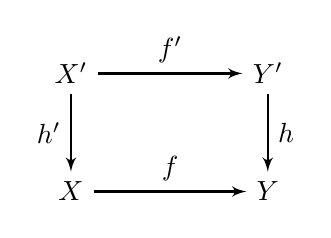
\begin{tikzpicture}
		[baseline=(current  bounding  box.center),thick,>=\arrtip]
		\node (a) at (0,0) {$X'$};
		\node (b) at (2.5,0) {$Y'$};
		\node (c) at (0,-1.5) {$X$};
		\node (d) at (2.5,-1.5) {$Y$};
		\draw[->] (a) to node[above] {$f' $} (b);
		\draw[->] (b) to node[right] {$h $} (d);
		\draw[->] (a) to node[left] {$h' $}(c);
		\draw[->] (c) to node[above] {$f $} (d);
	\end{tikzpicture}
\end{equation*}

\section{Lecture 1 (Monday)}
% !TeX root = LAWRGe2023Notes.tex

Hey this happened on Monday at 9 

\section{Lecture 2 (Monday)}
% !TeX root = LAWRGe2023Notes.tex

\documentclass[10pt]{amsart}

\newcommand{\B}{\mathrm{B}}
\newcommand{\C}{\mathbf{C}}
\newcommand{\rC}{\mathrm{C}}
\newcommand{\CP}{\mathbf{CP}}
\newcommand{\bE}{\mathbb{E}}
\newcommand{\rH}{\mathrm{H}}
\newcommand{\cO}{\mathcal{O}}
\newcommand{\bP}{\mathbb{P}}
\newcommand{\R}{\mathbf{R}}

\newcommand{\Conf}{\mathrm{Conf}}
\newcommand{\Emb}{\mathrm{Emb}}
\newcommand{\pt}{\mathrm{pt}}
\newcommand{\SO}{\mathrm{SO}}

\DeclareMathOperator{\Spec}{Spec}

\newcommand{\defterm}[1]{\textbf{\emph{#1}}}

\usepackage{tikz}
\usepackage{bbm}
\usetikzlibrary{3d,arrows,calc,positioning,decorations.pathreplacing,matrix}

\usepackage{calligra,mathrsfs}
\usepackage[all]{xy}
\usepackage{float, comment}
\usepackage{mathtools}
\usepackage{amsmath}
\usepackage{amsthm}
\usepackage{amssymb}
\usepackage{amsbsy}
\usepackage{amstext}
\usepackage{amsopn}
\usepackage[mathscr]{eucal}
\usepackage{enumerate}
\usepackage{xcolor}
\usepackage{graphicx}
\usepackage{scalerel}
\usepackage{microtype}
\usepackage[margin=1in,marginparwidth=0.8in, marginparsep=0.1in]{geometry}
\renewcommand{\baselinestretch}{1.2}
\usepackage[bookmarks=true, bookmarksopen=true, bookmarksdepth=3,bookmarksopenlevel=2, colorlinks=true, linkcolor=blue, citecolor=blue, filecolor=blue, menucolor=blue, urlcolor=blue]{hyperref}
\usepackage{xspace}

\DeclareMathOperator{\cHom}{\mathscr{H}\text{\kern -3pt {\calligra\large om}}\,}

\theoremstyle{definition}
\newtheorem{exercise}{Exercise}
\newtheorem*{Solution}{Solution}

\def\H{{H}}
\def\mod{{\rm{mod}}}
\def\res{{\rm{res}}}
\def\cl{{\mathrm{cl}}}
\def\cn{\leq 0}
\def\uk{\underline{k}}
\def\ti{{\tilde{i}}}
\def\tj{{\tilde{j}}}
\def\tm{{\tilde{m}}}
\def\tn{{\tilde{n}}}
\def\tp{{\tilde{p}}}
\def\tq{{\tilde{q}}}
\def\ts{{\tilde{s}}}
\def\n{{\bf{n}}}
\def\bL{{\mathbb{L}}}
\def\ua{{\underline{a}}}
\def\ub{{\underline{b}}}
\def\ue{{\underline{e}}}
\def\uj{{\underline{j}}}
\def\ux{{\underline{x}}}
\def\uy{{\underline{y}}}
\def\la{\langle}
\def\ra{\rangle}
\def\ov{\overline}
\def\ul{\underline}
\def\wt{\widetilde}

\def\ba{\begin{align}}
\def\ea{\end{align}}

\def\be{\begin{equation}}
\def\ee{\end{equation}}

\def\bc{\begin{center}}
\def\ec{\end{center}}

\def\bp{\begin{proof}}
\def\ep{\end{proof}}

\def\bi{\begin{itemize}}
\def\ei{\end{itemize}}

\def\ben{\begin{enumerate}}
\def\een{\end{enumerate}}

\def\bt{\begin{tabular}}
\def\et{\end{tabular}}

\def\i{\item}

\def\lra{\longrightarrow}
\def\Lra{\Longrightarrow}
\def\iff{\Leftrightarrow}

\newcommand{\Z}{\mathbf{Z}}
\newcommand{\cA}{\mathcal{A}}
\newcommand{\cB}{\mathcal{B}}
\newcommand{\cC}{\mathcal{C}}
\newcommand{\Q}{\mathbf{Q}}
\newcommand{\arrtip}{latex'}

\theoremstyle{definition}
\newtheorem{defn}[thm]{Definition}

\begin{document}
\title{Algebraic structures in TQFTs}
\author{Pavel Safronov}
\maketitle

In this lecture $Z$ denotes some $d$-dimensional TQFT. For simplicity I will assume that it is fully extended, but many statements make sense with partially extended TQFTs. I will assume that the TQFT is valued in the ($\infty$-)category of chain complexes.

\section{Local and line operators}

Besides computing partition functions, in physics one is often interested in computing correlation functions of some local operators. Let us introduce them using the following heuristic idea.

Suppose $M$ is a closed oriented $d$-manifold and $x\in M$ is a point with an insertion of a ``local operator'' $\cO$. By locality one should be able to compute the partition function as follows:
\begin{itemize}
\item Consider a ball $D\subset M$ around $x$ and let $S^{d-1}\subset M$ be its boundary.
\item $Z(M\setminus D)$ defines a map $Z(S^{d-1})\rightarrow \C$. The local operator defines a map $Z(D_{\cO})\colon \C\rightarrow Z(S^{d-1})$ and the partition function on $M$ is the composite of these two maps.
\end{itemize}

If we are being agnostic about local operators, we may observe that the only thing we have used about them is the vector of $Z(S^{d-1})$ that they define. This leads us to the following definition.

\begin{defn}
Let $Z$ be a $d$-dimensional TQFT. The \defterm{space of local operators} is the chain complex $Z(S^{d-1})$.
\end{defn}

One also considers defects given by extended objects: lines, surfaces, ... embedded in $M$. Besides local operators, we will only encounter line operators this week. We can think of them as follows:
\begin{itemize}
\item A line operator is specified by a defect supported on a knot $K\subset M$. The same analysis as before shows that we can compute the partition function if we know the corresponding vector in $Z(S^{d-2}\times K)$.

\item One often only considers ``local'' line operators which themselves obey cutting and gluing axioms of a TQFT. These local line operators define an object of the category $Z(S^{d-2})$.
\end{itemize}

This motivates the following definition.

\begin{defn}
Let $Z$ be a $d$-dimensional TQFT.
\begin{itemize}
\item The \defterm{space of line operators} is $Z(S^{d-2}\times S^1)$.
\item The \defterm{category of line operators} is $Z(S^{d-2})$.
\end{itemize}
\end{defn}

\section{$\bE_d$-algebras}

Our next goal is to explain algebraic structures present on the space of local and line operators. Given any cobordism $W$ from $k$ copies of $S^{d-1}$ to $S^{d-1}$ we get an algebraic operation
\[Z(W)\colon Z(S^{d-1})^{\otimes k}\longrightarrow Z(S^{d-1})\]
on the space of local operators in any TQFT. We will now investigate operations coming from cobordisms ``with no topology''.

\begin{defn}
Fix a dimension $d$.
\begin{itemize}
\item \[\bE_d(k) = \Emb^{fr}(D^{\coprod k}, D)\]
is the space of (smooth) framed embeddings of $k$ $d$-dimensional open disks $D$ into a given disk $D$.

\item \[\bE^{fr}_d(k) = \Emb(D^{\coprod k}, D)\]
is the space of (smooth) oriented embeddings of $k$ $d$-dimensional open disks $D$ into a given disk $D$.
\end{itemize}
\end{defn}

There are natural composition maps which make $\bE_d$ and $\bE^{fr}_d$ into operads. In particular, we can talk about their algebras.

\begin{example}
The operads $\bE_1$ and $\bE^{fr}_1$ are both equivalent to the associative operad.
\end{example}

\begin{example}
There is a natural action of $\SO(d)$ on $\bE_d$, so that a $\bE^{fr}_d$-algebra is an $\bE_d$-algebra equipped with a compatible $\SO(d)$-action.
\end{example}

Given an embedding $D^{\coprod k}\hookrightarrow D$ we obtain a cobordism from $(S^{d-1})^{\coprod k}$ to $S^{d-1}$ by removing the interiors of the embedded disks. In particular, we obtain a natural map
\[\rC_\bullet(\bE^{fr}_d(k); \C)\otimes_\C Z(S^{d-1})^{\otimes k}\longrightarrow Z(S^{d-1})\]
for any oriented TQFT. Similarly, if $Z$ is a framed TQFT we get a natural map
\[\rC_\bullet(\bE_d(k); \C)\otimes_\C Z(S^{d-1})^{\otimes k}\longrightarrow Z(S^{d-1}).\]
Both maps are compatible with compositions and we obtain the following result:
\begin{itemize}
\item If $Z$ is a framed TQFT, the chain complex of local operators $Z(S^{d-1})$ is an $\bE_d$-algebra.
\item If $Z$ is an oriented TQFT, the chain complex of local operators $Z(S^{d-1})$ is a framed $\bE_d$-algebra.
\end{itemize}

Up to homotopy the spaces of embeddings may be identified as follows.

\begin{prop}
There are homotopy equivalences
\[\bE_d(k)\cong \Conf_k(\R^d),\qquad \bE^{fr}_d(k)\cong \SO(d)^k\times \Conf_k(\R^d),\]
where $\Conf_k(\R^d)$ is the configuration space of $k$ distinct ordered points in $\R^d$.
\end{prop}

Using the above description one can show the following:
\begin{itemize}
\item An $\bE_2$-algebra in categories is a braided monoidal category.
\item An $\bE^{fr}_2$-algebra in categories is a balanced monoidal category, i.e. there is an extra automorphism of the identity functor, the \emph{balancing} $\theta$, which satisfies
\[\theta_{x\otimes y} = \sigma_{y, x}\circ \sigma_{x, y}\circ (\theta_x\otimes \theta_y).\]
\end{itemize}

So, the category of line operators in a 3-dimensional TQFT is a balanced monoidal category.

\section{$\bP_d$-algebras}

To describe $\bE_d$-algebras in chain complexes, let us first introduce a related notion.

\begin{defn}
A \defterm{$\bP_d$-algebra} is a commutative dg algebra $A$ equipped with a bracket of cohomological degree $1-d$ (inducing a Lie structure on $A[d-1]$) satisfying the Leibniz rule
\[\{a, bc\} = \{a, b\}c + (-1)^{|b||c|}\{a, c\}b\]
for $a,b,c\in A$.
\end{defn}

\begin{remark}
A $\bP_2$-algebra is known as a \emph{Gerstenhaber algebra}.
\end{remark}

Let $\bP_d(k)$ be the vector space of all operations $A^{\otimes k}\rightarrow A$ on a $\bP_d$-algebra. We can formalize it as follows: define $\bP_d(k)$ to be the subspace of the free $\bP_d$-algebra on degree 0 variables $x_1, \dots, x_k$ consisting of expressions where each $x_i$ appears exactly once. For instance:
\begin{itemize}
\item $\bP_d(1)\cong \C$ spanned by the identity map $A\rightarrow A$.
\item $\bP_d(2)\cong \C\oplus \C[d-1]$ spanned by the commutative multiplication $m\colon A\otimes A\rightarrow A$ and $\{-, -\}\colon A\otimes A\rightarrow A[1-d]$ by the Poisson bracket.
\end{itemize}

We have the following claim.

\begin{defn}
Suppose $d\geq 2$. Then there is an isomorphism of graded vector spaces $\rH_\bullet(\bE_d(k); \C)\cong \bP_d(k)$.
\end{defn}

\begin{remark}
In fact, both $\bE_d$ and $\bP_d$ are operads and there is an equivalence $\rC_\bullet(\bE_d; \C)\cong \bP_d$ of graded linear operads.
\end{remark}

As a corollary, given an $\bE_d$-algebra $A$, its homology $\rH_\bullet(A)$ has a natural structure of a $\bP_d$-algebra.

\begin{example}
Let $Z$ be a 3d TQFT. Then the cohomology of the space of local operators $\rH^\bullet(Z(S^2))$ carries a graded commutative multiplication as well as Poisson bracket of degree $-2$.
\end{example}

\section{$\Omega$-deformation}

We will now explain an important construction with $\bE_d$-operads which is known in physics as the procedure of $\Omega$-deformation.

Consider the $\bE_d$-operad equipped with its natural $\SO(d)$-action. There is a natural inclusion of operads $\bE_{d-2}\hookrightarrow \bE_d$ which is $\SO(d-2)\times \SO(2)$-equivariant, where the $\SO(2)$-action on the left is trivial.

\begin{thm}
The inclusion of operads $\bE_{d-2}\hookrightarrow \bE_d$ realizes $\bE_{d-2}$ as the space of fixed points of the $\SO(2)$-action on $\bE_d$.
\label{thm:Enfixedpoints}
\end{thm}

To state an important corollary, let us first recall a few basics of equivariant localization. Given a space $X$ with an action of a topological group $G$ we may consider equivariant homology $\rH^G_\bullet(X)$ and cohomology $\rH^\bullet_G(X)$ which are both modules over $\rH^\bullet_G(\pt)=\rH^\bullet(\B G)$.

\begin{example}
We have $\B\SO(2)=\CP^\infty$, so $\rH^\bullet(\B\SO(2))=\C[\epsilon]$, where $\deg(\epsilon)=2$.
\end{example}

\begin{thm}[Equivariant localization]
Let $G$ be a topological group. Let $Y$ be a space with a $G$-action. Let $X$ be a topological space equipped with a trivial $G$-action and a $G$-equivariant map $X\rightarrow Y$ which realizes $X$ as the space of fixed points of the $G$-action on $Y$. Then the induced map
\[\rH^G_\bullet(X)\otimes_{\C[\epsilon]} \C(\epsilon) \longrightarrow \rH^G_\bullet(Y)\otimes_{\C[\epsilon]} \C(\epsilon)\]
is an isomorphism.
\end{thm}

Combining the theory of equivariant localization and \cref{thm:Enfixedpoints} we get the following.

\begin{thm}
Let $A$ be a framed $\bE_d$-algebra. Consider the induced $\SO(2)\subset\SO(d)$-action on $A$. Then $A^{\SO(2)}\otimes_{\C[\epsilon]} \C(\epsilon)$ is a framed $\bE_{d-2}$-algebra.
\end{thm}

\begin{example}
Let $Z$ be a 3d TQFT and consider the framed $\bE_3$-algebra structure on the space of local operators $Z(S^2)$. Recall that its cohomology $\rH^\bullet(Z(S^2))$ carries a natural (graded) Poisson structure. The equivariant localization
\[\rH^\bullet_{\SO(2)}(Z(S^2))\otimes_{\C[\epsilon]} \C(\epsilon)\]
is an associative algebra which provides a deformation quantization of $\rH^\bullet(Z(S^2))$ (with the quantization parameter being $\epsilon$).
\end{example}

\section{Swiss-cheese algebras}

I will end this lecture by describing algebraic structures appearing in TQFTs with boundary conditions.

Let $Z$ be a $d$-dimensional TQFT with a chosen boundary condition $Z^\partial$. We can extract the following kinds of algebras:
\begin{itemize}
\item The space of \emph{bulk local operators} in $Z$, i.e.
\[A = Z(S^{d-1}),\]
carries the structure of a framed $\bE_d$-algebra.

\item The space of \emph{boundary local operators}, i.e.
\[B = Z(D^{d-1})(Z^\partial(S^{d-2})),\]
carries the structure of a framed $\bE_{d-1}$-algebra. Namely, let $H$ be the $d$-dimensional half-ball. Consider the space
\[\Emb^\partial(H^{\coprod k}, H)\]
of oriented embeddings of $k$ $d$-dimensional half-balls into a single one so that the boundaries are embedded into the boundaries. Retracting the half-ball to its boundary (a $(d-1)$-dimensional ball) identifies this space with $\bE^{fr}_{d-1}$.

\item In addition, there is an action of $A$ on $B$ as follows. Let $D$ be a $d$-dimensional ball and $H$ a $d$-dimensional half-ball. Any embedding $D^{\coprod l}\coprod H^{\coprod k}\hookrightarrow H$ (so that the boundaries of the half-balls are embedded in the boundary of the bigger half-ball) gives rise to an operation
\[A^{\otimes l}\otimes B^{\otimes k}\longrightarrow B.\]
\end{itemize}

The pair $(A, B)$ together with the operations described above is known as a $d$-dimensional \defterm{Swiss-cheese algebra}. We will encounter the following manifestation of this structure.

\begin{example}
Let $Z$ be a 3d TQFT with a boundary condition $Z^\partial$. Let $A$ be the $\bE_3$-algebra of bulk local operators and $B$ the $\bE_2$-algebra of boundary local operators. $A$ carries a degree $-2$ Poisson structure. There is a map of graded commutative algebras $A\rightarrow B$ and the induced map $\Spec B\rightarrow \Spec A$ is coisotropic.
\end{example}

\begin{remark}
There is a homotopy notion of a coisotropic submanifold which is precisely defined in terms of a Swiss-cheese algebra structure.
\end{remark}


Recall that $\bE_n(k)$ is homotopy equivalent to $\Conf_k(\R^n)$, the configuration space of $k$ distinct points in $\R^n$.

Recall that a $\bP_n$-algebra is a dg commutative algebra $A$ equipped with a bracket $\{-, -\}$ of cohomological degree $1-n$ (inducing a Lie structure on $A[n-1]$) satisfying the relation $\{a, bc\} = \{a, b\}c + (-1)^{|b||c|}\{a, c\}b$. Let $\bP_n(k)$ be the subspace of the free $\bP_n$-algebra on degree $0$ variables $x_1, \dots, x_k$ consisting of expressions where each $x_i$ appears exactly once. For instance, $\{\{x_1, x_2\}, \{x_3, x_4\}\}$ is an element of $\bP_n(4)$ of cohomological degree $3(1-n)$.

\section{Exercises}
\begin{exercise}
Consider the map $\Conf_k(\R^n)\rightarrow \Conf_{k-1}(\R^n)$ given by forgetting the last point. Show that its fiber $F_k$ is homotopy equivalent to a wedge of $(k-1)$ spheres $S^{n-1}$.
\end{exercise}

\begin{exercise}
The Leray--Serre spectral sequence for the fibration $F_k\hookrightarrow \Conf_k(\R^n)\rightarrow \Conf_{k-1}(\R^n)$ degenerates (using the Leray--Hirsch theorem), so that one may identify
\[\rH_\bullet(\Conf_k(\R^n);\Q)\cong \rH_\bullet(\Conf_{k-1}(\R^n);\Q)\otimes \rH_\bullet(F_k;\Q).\]
Find $\rH_\bullet(\bE_n(k);\Q)$ for $k=1,2,3$.
\end{exercise}

\begin{exercise}
Describe the graded vector space $\bP_n(k)$ for $k=1,2,3$ and find an isomorphism
\[\rH_\bullet(\bE_n(k);\Q)\cong \bP_n(k)\]
for $n\geq 2$.
\end{exercise}

\begin{exercise}
(*) Consider the $S_2$-action on $\bE_2(2)\sim S^1$ given by reflection around the origin. Let $\cC$ be a category. Show that an $S_2$-equivariant map
\[S^1\times \cC^{\times 2}\longrightarrow \cC\]
is the same as a pair $(\otimes, \sigma)$ consisting of a functor $\otimes\colon \cC\times \cC\rightarrow \cC$ as well as a natural isomorphism
\[\sigma_{x, y}\colon x\otimes y\xrightarrow{\sim} y\otimes x.\]
\end{exercise}

\end{document}


\section{Lecture 3 (Monday)}
% !TeX root = LAWRGe2023Notes.tex


\subsection{Supersymmetry}
My goals for this talk are to give an answer to the questions ``what is supersymmetry?'' and ``what is a topological twist?''.

We're going to be working in the wide world of models for classical and quantum field theory.  I won't explain in detail what a quantum field theory is, and there are many different ways of modelling them, but part of the data will be a vector space (either of states, or of observables).  In fact, usually a little more, a cochain complex $(\mathcal E, \mathrm{d})$.  We can ask for $\mathcal E$ to be acted upon by some Lie algebra $\mathfrak{g}$ of symmetries.
\begin{example} If we're studying field theory on $\RR^4$, we might ask for an action of the Lorentz algebra $\so(1,3)$.  Or of the associated Poincar\'e algebra $\mathfrak{iso}(1,3) = \so(1,3) \ltimes \RR^4$. \end{example}

The term \emph{supersymmetry} is used for an enhancement of this sort of thing, where the Poincar\'e algebra is replaced by a $\ZZ/2\ZZ$-graded extension thereof.
\begin{Definition}
	A \emph{super Lie algebra} is a $\ZZ/2\ZZ$-graded vector space $\mathfrak{g}$ equipped with a Lie bracket that is graded skew-symmetric:
	\[[X,Y] = (-1)^{|X||Y|+1}[Y,X]\]
	and satisfies the graded Jacobi identity
	\[(-1)^{|X||Z|}[X,[Y,Z]] + (-1)^{|Y||X|}[Y,[Z,X]] + (-1)^{|Z||Y|}[Z,[X,Y]] = 0.\]
	here $|X| \in \ZZ/2\ZZ$ denotes the degree of an element $X \in \mathfrak{g}$.
\end{Definition}
We will now define the super Lie algebras where supersymmetries live.  For simplicity we will focus on the \emph{complexified} Lie algebra of supersymmetries, which will be an extension of $\mathfrak{iso}(n,\CC) = \mathfrak{iso}(p,q) \otimes_\RR \CC$ for any $p+q=n$.
\begin{Definition}
	A \emph{super Poincar\'e algebra} in dimension $n$ is a super Lie algebra with underlying super vector space
	\[\mathfrak{siso}(n|\Sigma) = \mathfrak{iso}(n,\CC) \oplus \Pi \Sigma\]
	(where $\Pi$ indicates an odd degree shift), where $\Sigma$ is a \emph{spinorial} representation of $\so(n,\CC)$ (meaning all its irreducible summands are (semi)spin representations of $\so(n,\CC)$), with an additional bracket given by a non-degenerate equivariant map $\Gamma \colon \sym^2(\Sigma) \to \CC^n$.
\end{Definition}

\begin{remark}
	We could of course also study the real forms of these complex super Lie algebras, which will depend on a choice of signature.  We won't need these real forms this week.
\end{remark}

So we can now say what a supersymmetric field theory is (subject to the caveat that we haven't exactly defined a field theory, only stated that its structure should include a cochain complex!)
\begin{Definition}
	Suppose that $(\mathcal E,\mathrm{d})$ is a classical field theory on $\RR^n$ with an action of the algebra $\mathfrak{iso}(n,\CC)$ of isometries.  We say $(\mathcal E,\mathrm{d})$ is \emph{supersymmetric} with supersymmetry $\Sigma$ if $\mathcal E$ is equipped with an additional $\ZZ/2\ZZ$-grading (as well as its original $\ZZ$-grading) and the $\mathfrak{iso}(n,\CC)$ lifts to an action of the super Lie algebra $\mathfrak{siso}(n|\Sigma)$.
\end{Definition}

You might notice that we typically use slightly different terminology.  We don't usually talk about ``supersymmetry $\Sigma$'', we usually say something like ``$\mathcal N=2$ supersymmetry'' or ``$\mathcal N=4$ supersymmetry'' or $\mathcal N=(2,2)$ supersymmetry''.  We'll explain this now: it's because the possible odd terms $\Sigma$ occuring in the supersymmetry algebra are generally highly constrained.  They are given as sums of irreducible spinorial representations of which there are always either one or two.  The bracket $\Gamma$ of odd elements is also usually uniquely determined, maybe up to an overall scale.  This is why it didn't appear in our notation.

\begin{example}[3d supersymmetry]
	The key example this week is supersymmetry in 3d, so let's do this example first.  As I mentioned, for simplicity I'm going to complexify my super Poincar\'e algebras, and the vector spaces $\mathcal E$ on which they act, that way I won't have to worry about a choice of signature.
	
	Recall that there is an exceptional isomorphism $\spin(3,\CC) \cong \SL(2,\CC)$ (or perhaps more familiarly, in Euclidean signature $\spin(3) \cong \SU(2)$).  The finite-dimensional irreducible representations of $\SL(2,\CC)$ or its Lie algebra $\sl(2,\CC)$ are given as $\sym^k(V)$, where $V$ is the 2d defining representation.  In particular, the 3d defining representation of $\so(3,\CC)$ is isomorphic to $\sym^2(V)$.
	
	The spin representation is, under this isomorphism, $V$ itself, so there are potentially super Poincar\'e algebras with $\Sigma = V^k = V \otimes W$ where $W$ is a $k$-dimensional vector space, for $k \ge 1$.  To work out the possible brackets, we need an equivariant map
	\[\sym^2(\Sigma) = \sym^2(V \otimes W) = \sym^2(V) \otimes\sym^2(W) \oplus \wedge^2(V) \otimes \wedge^2(W) \to \sym^2(V).\]
	So pretty clearly we get such a map for any linear map $g \colon \sym^2(W) \to \CC$, and non-degeneracy of the bracket means $g$ is precisely an inner product on $W$.
	
\end{example}

This example also illustrates an important concept: there are symmetries of the super Poincar\'e algebra in dimension 3 coming from elements of $\mathrm O(W)$.  These are called \emph{R-symmetries}.

\begin{Definition}
	The group $G_R$ of \emph{R-symmetries} of a super Poincar\'e algebra is the group of outer automorphisms of $\mathfrak{siso}(n|\Sigma)$ that act trivially on the even part.  Write $\mathfrak{g}_R$ for its Lie algebra.
\end{Definition}

\begin{remark}
	If we like we can form the extension $\mathfrak{g}_R \ltimes \mathfrak{siso}(n|\Sigma)$ by the algebra of R-symmetries (or a subalgebra thereof).  Such super Lie algebras are sometimes more generally referred to as ``supersymmetry algebras''.
\end{remark}

\subsection{Twisting}
To conclude, I'd like to talk about the concept of ``twisting''.  Suppose $Q \in \mathfrak{siso}(n|\Sigma)$ is an odd element such that $[Q,Q]=0$.  If $\mathcal E$ is a supersymmetric theory, we can use such a ``square-zero'' element $Q$ to define a deformation to a new theory.
\begin{Definition}
	Let $(\mathcal E,\mathrm{d})$ be a supersymmetric theory, and write $\alpha$ for the action of $\mathfrak{siso}(n|\Sigma)$ on $\mathcal E$.  The \emph{twist} of $(\mathcal E,\mathrm{d})$ by a square-zero element $Q$ is the theory $(\mathcal E_!,\mathrm{d}_Q) = (E, \mathrm{d} + \alpha(Q))$.
\end{Definition}
The square-zero condition is needed to ensure that $\mathrm{d}_Q$ is indeed a differential.  Notice that $\mathrm{d}_Q$ is not of homogeneous degree anymore, so in general $(\mathcal E, \mathrm{d} + \alpha(Q))$ is only a $\ZZ/2\ZZ$-graded complex (though in many examples it is possible to cook up a $\ZZ$-grading after all!).

So, if we are studying twists, it is natural to ask exactly what sorts of elements $Q$ we can twist by!  Those elements satisfying the quadratic equation $[Q,Q]$ cut out a quadric subvariety of $\Sigma$.
\begin{Definition}
	The \emph{nilpotence variety} associated to a super Poincar\'e algebra with odd summand $\Sigma$ is the subvariety
	\[\mathcal N\mathrm{ilp} = \{Q \colon [Q,Q] = 0\} \subseteq\Sigma.\]
	Notice that $\mathcal N\mathrm{ilp}$ is invariant under the rescaling action of $\CC^\times$, by $Q \mapsto \lambda Q$.  So we can instead study the projectivization of $\mathcal N\mathrm{ilp}$:
	\[\mathbb P \mathcal N \mathrm{ilp}= (\mathcal N\mathrm{ilp} \backslash \{0\})/\CC^\times \subseteq\mathbb P \Sigma.\]
\end{Definition}

You'll work through an example in detail during the exercise session shortly: the example of 3d $\mathcal N=4$ supersymmetry that is most relevant to this week's lectures.

\subsection{Twisting and Translation Invariance}
Let us conclude by talking about what twisting ``buys us''.  In what sense are twists of supersymmetric theories more mathematically tractable?  Well, in many cases, they are in fact topological!  Here's the idea.

Suppose that our field theory $\mathcal E$ can be equipped with a Lie bracket for which the action of $\mathfrak{siso}(n|\Sigma)$ is \emph{inner}.  In other words, suppose that there is a Lie algebra map
\[H \colon \mathfrak{siso}(n|\Sigma) \to \mathcal E\]
so that the action of $X \in \mathfrak{siso}(n|\Sigma)$ coincides with the Lie bracket with $H(X) \in \mathcal E$ (these elements $H(X)$ are the \emph{Hamiltonians} of the symmetries $X$).  What happens in the twist $\mathcal E_Q$?  Well, for any $Q$-exact symmetry $X = [Q,Q']$, the Hamiltonian $H(X)$ is \emph{cohomologically trivial} in the twist by $Q$.

The image $\mathfrak b_Q$ of $[Q,-]$ is a subalgebra of the abelian Lie algebra $\CC^n$ of translations.  So this is saying that certain translations act cohomologically trivially in the twisted theory.  If $\mathfrak b_Q = \CC^n$ contains \emph{all} translations then we say $Q$ is a \emph{topological supercharge}.  It turns out, that under some fairly mild assumptions, the twist by a topological supercharge is always a topological field theory!

In the exercise session you will show that there are two inequivalent families of topological supercharges in the 3d $\mathcal N=4$ nilpotence variety.

\subsection{Exercises}
In this exercise we will learn about twists in a three-dimensional example. Recall that $\spin(3, \CC) \cong \SL(2, \CC)$. Let $S$ be the two-dimensional spin representation of $\spin(3, \CC)$ (i.e. the defining representation of $\SL(2, \CC)$) and $V$ the three-dimensional vector representation (i.e. the adjoint representation of $\SL(2, \CC)$). There is an isomorphism $\sym^2(S)\cong V$ of $\spin(3, \CC)$-representations.

Spinorial representation take the form $\Sigma = S\otimes W$, where $W$ is a complex vector space equipped with a nondegenerate symmetric bilinear pairing $g$. The super Poincar\'e Lie algebra is
\[\mathfrak{siso}(3|\Sigma) = \mathfrak{iso}(3,\CC)\oplus \Pi \Sigma\]
with the only nonobvious bracket $\Gamma\colon \sym^2(\Sigma)\rightarrow V$ defined using $g$ and the isomorphism $\sym^2(S)\cong V$.  The R-symmetry group here is the group $\mathrm O(W)$ acting on $W$.

Consider the case $\dim W = 4$, i.e. we are working with 3d $\mathcal N=4$ supersymmetry.

\begin{enumerate}
	\item For a basis $\{Q_1,Q_2\}$ of $S$ let $Q=Q_1\otimes u + Q_2\otimes v\in\Sigma$. Give conditions under which $Q$ lies in the nilpotence variety $\mathcal N$.
	
	\item What are the $\Spin(3, \CC) \times \SO(W)$-orbits in the nilpotence variety $\mathcal N$ and its projectivization $\mathbb {P}\mathcal N$? (\emph{Hint}: there are 3 orbits in the latter case.)
	
	\item Let $\mathfrak b_Q\subset V$ be the image of $\Gamma(Q, -)\colon \Sigma\rightarrow V$. Find the dimension of $\mathfrak b_Q$ for an element $Q$ in each orbit.
	
	\item (*) Let $\mathfrak z_Q\subset \mathfrak{siso}(3|\Sigma)$ be the subalgebra of elements commuting with $Q$. This subalgebra has a nice interpretation: it consists of those symmetries that ``survive'' the twist, i.e. that continue to act on the twisted theory. Find this subalgebra for each orbit.
\end{enumerate}

\begin{remark}
	The moduli space $\mathrm{OGr}(1, 4)$ of isotropic lines in $W$ is a nondegenerate quadric surface in $\mathbb P(W) \cong \mathbb{CP}^3$ and therefore is isomorphic to $\mathbb{CP}^1\times\mathbb{CP}^1$.
\end{remark}

\begin{remark}
	The moduli space $\mathrm{OGr}(2, 4)$ of isotropic planes in $W$ is isomorphic to the moduli space of lines in $\mathrm{OGr}(1, 4)$ by the map sending an isotropic plane $\Pi \subseteq W$ to the family of lines $L \subseteq\Pi$, which are automatically all isotropic. This moduli space of lines, and hence the moduli space $\mathrm{OGr}(2,4)$, is isomorphic to $\mathbb{CP}^1\sqcup\mathbb{CP}^1$.  Given a point $P\in\mathbb{CP}^1$ there are two lines $P\times \mathbb{CP}^1\subset \mathrm{OGr}(1, 4)$ and $\mathbb{CP}^1\times P\subset \mathrm{OGr}(1, 4)$.
\end{remark}


\section{Lecture 4 (Monday)}
% !TeX root = LAWRGe2023Notes.tex

Hey this happened on Monday at 9 

\section{Lecture 5 (Tuesday)}
% !TeX root = LAWRGe2023Notes.tex

Hey this happened on Monday at 9 

\section{Lecture 6 (Tuesday)}
% !TeX root = LAWRGe2023Notes.tex

%\title{Reidemeister torsion and the Meng--Taubes--Turaev theorem}
%\author{Pavel Safronov}
%\maketitle
\newcommand{\id}{\mathrm{id}}
\newcommand{\bH}{\mathbf{H}}
\newcommand{\fs}{\mathfrak{s}}
If $M$ is a complex manifold, the partition function of the 2d B-model with target $M$ as well as the partition function of the 3d B-model with target $\T^* M$ are both given by Reidemeister torsion. In this lecture we introduce what it is as well as state the first example of a mirror symmetry phenomenon.

\subsection{Torsion}

Let $R$ be a commutative ring with a homomorphism $R\rightarrow K$ to a field $K$. Let $N$ be a connected finite CW complex (let $x\in N$ be a chosen basepoint) and $\cL$ a free $R$-module of finite rank equipped with a $\pi_1(N)$-action. It defines a homomorphism
\[\pi_1(N)\longrightarrow \GL_n(R)\]
and hence a homomorphism
\[\det\colon \rH_1(N;\Z)\longrightarrow K^\times\]
by post-composing the first map with $\GL_n(R)\rightarrow \GL_n(K)\xrightarrow{\det} K^\times$.

Let $\tilde{N}\rightarrow N$ be the universal cover (with its natural $\pi_1(N)$-action) and lift the CW structure from $N$ to $\tilde{N}$. Consider the complex of cellular chains
\[\rC_0(\tilde{N}; \Z)\xleftarrow{d} \rC_1(\tilde{N}; \Z)\xleftarrow{d} \dots\]
as a complex of $\pi_1(N)$-representations. Applying $\otimes_{\Z[\pi_1(N)]}\cL$ we get the complex of cellular chains
\[\rC_0(N; \cL)\xleftarrow{d} \rC_1(N; \cL)\xleftarrow{d} \dots\]

Assume that this complex is acyclic when we apply $\otimes_R K$. Over a field an acyclic complex is contractible, so there is a contracting homotopy $h$ (defined over $K$).

\begin{defn}
	Let $N$ be a connected finite CW complex with a chosen basepoint $x\in N$. A \defterm{Turaev spider} $\fs$ is a choice of a path from the center of each cell to $x$.
\end{defn}

Note that given two spiders $\fs_1,\fs_2$, we may measure their difference $\fs_1-\fs_2\in\rH_1(N;\Z)$ as follows. The difference of two paths from $\sigma\in A_d$ to $x$ gives an element of $\rH_1(N; \Z)$; $\fs_1-\fs_2$ is defined to be an alternating sum of these differences over each cell. We say two Turaev spiders are equivalent if the difference between them gives the zero element of $\rH_1(N; \Z)$.

\begin{prop}[Turaev]
	Let $N$ be a closed oriented 3-manifold. There is a natural bijection between the set of Turaev spiders and the set of $\Spin^c$-structures. This bijection is equivariant for the action of $\rH_1(N; \Z)\cong\rH^2(N; \Z)$.
\end{prop}

Choose a basis of $\cL$, an ordering of cells and a Turaev spider $\fs$. The Turaev spider allows us to produce a canonical lift $\tilde{\sigma}$ to a cell of $\tilde{N}$ of each cell $\sigma$ of $N$. Therefore, the complex of cellular chains $\rC_\bullet(N; \cL)$ becomes a complex of free finite rank modules
\[R^{n_1}\xleftarrow{d} R^{n_2}\xleftarrow{d} \dots\]

Consider the map $d+h\colon \rC_{even}(N; \cL)\otimes_R K\rightarrow \rC_{odd}(N; \cL)\otimes_R K$. Since the complex of cellular chains is acyclic over $K$, this map is invertible. In particular, we can compute its determinant
\[\det(d + h)\in K^\times.\]
Let us analyze how this element changes if we make different choices:
\begin{itemize}
	\item Reordering the cells introduces a sign ambiguity into $\det(d + h)$.
	
	\item Changing the basis of $\cL_x$ changes $\det(d+h)$ by a unit of $R$.
	
	\item Changing the Turaev spider changes $\det(d+h)$ by the image of
	\[\det\colon \rH_1(N; \Z)\longrightarrow K^\times.\]
\end{itemize}

So, from this setup we get an element
\[\det(d + h)\in K^\times / R^\times.\]

\subsection{Milnor torsion}

Let us now specialize the discussion. Let $H=\rH_1(N; \Z)/\{torsion\}$, $R=\Z[H]$ and $K = \Q(H)$. We have $R^\times = \pm H$. Let $\cL = \Z[H]$ equipped with the obvious homomorphism $\pi_1(M)\rightarrow \rH_1(N; \Z)
\rightarrow H\rightarrow \Z[H]$.

\begin{defn}
	The \defterm{Milnor torsion} $\tau(N)$ of $N$ is zero if the chain complex $\rC_\bullet(N; \cL)\otimes_R K$ is not acyclic and otherwise it is defined to be
	\[\det(d + h)\in \Q(H) / (\pm H).\]
\end{defn}

\begin{example}
	Consider the circle $N=S^1$. The Milnor torsion is
	\[\tau(S^1) = \frac{1}{1-t}\in\Q(t)/(\pm t^\Z).\]
\end{example}

Let us now indicate how to define torsion without the ambiguity of $\pm t^\Z$ (this is known as \emph{Turaev (or refined) torsion}):
\begin{itemize}
	\item The ambiguity of $t^\Z$ would be resolved if we choose a Turaev spider. A more homotopy-theoretic definition is as follows. For a finite CW complex $N$ there is the homological Euler class $e(N)\rH_0(N; \Z)$. A bounding chain for this class is known as the \defterm{Euler structure}.
	
	\item The sign ambiguity arose because we could reorder the cells. To fix this ambiguity we can fix an orientation of the determinant line of $\rH_\bullet(N;\R)$.
\end{itemize}

\subsection{Meng--Taubes--Turaev}

We are now ready to state one instance of 3-dimensional mirror symmetry. Let us recall that given the data of
\begin{itemize}
	\item A compact Lie group $G$.
	\item A quaternionic $G$-representation $W$.
\end{itemize}
there are 3-dimensional TQFTs $Z_{3dA, W/\!/\!/G}$ and $Z_{3dB, W/\!/\!/G}$. Moreover, if the pairs $(G, W)$ and $(G^\vee, W^\vee)$ are 3d mirror, we should have an equivalence of 3d TQFTs
\[Z_{3dA, W/\!/\!/G}\cong Z_{3dB, W^\vee/\!/\!/G^\vee}.\]
One basic example of 3d mirror symmetry we will often return to is the 3d mirror symmetry between $(\U(1), \bH)$ and $(\pt, \bH)$.

In particular, we expect an equality
\[Z_{3dA, \bH/\!/\!/\U(1)}(N) = Z_{3dB, \bH}(N)\]
of the partition functions of these TQFTs. We will not give all details, but:
\begin{itemize}
	\item The partition function of the 3d A-model for $(G, W)$ counts solutions of the Seiberg--Witten equations.
	\item The partition function of the 3d B-model for $(G, V\otimes_\C \bH)$ computes the integral of torsion over the moduli space of pairs of a flat $G_\C$-bundle $P$ on $N$ and a flat section of the associated bundle $P\times^{G_\C} V$.
\end{itemize}

In the simplest case $(\U(1), \bH)$ we are reduced to computing Seiberg--Witten invariants.

\begin{thm}[Meng--Taubes--Turaev]
	Let $N$ be a 3-manifold with $b_1(N)>1$. There is an equality
	\[\SW_N = \tau(N)\in\Z[H]/(\pm H).\]
\end{thm}

\begin{remark}
	Choosing a $\Spin^c$ structure $\sigma$ we can refine the statement to an equality
	\[\SW_N(\sigma) = \tau(N)\in\Z[H]/(\pm 1),\]
	where $\tau(N)$ is the refined torsion which depends on $\sigma$.
\end{remark}

\begin{remark}
	There are also more delicate statements when $b_1(N) = 1$ and $b_1(N)=0$. The problem with these cases is that the Seiberg--Witten invariants depend on perturbation and exhibit a wall-crossing behavior.
\end{remark}

\begin{exercise}
	Consider the cell structure on $N=S^1$ with one 0-cell and one 1-cell. In this case $\pi_1(N)=\rH_1(N;\Z)=H$ and $\Z[H]=\Z[t, t^{-1}]$.
	\begin{enumerate}
		\item Lift the cell structure on $N$ to a cell structure on the universal cover $\tilde{N}$.
		\item Show that the chain complex
		\[C_\bullet = \rC_\bullet(\tilde{N}; \Z)\otimes_{\Z[H]}\Q(H)\]
		is acyclic and find a contracting homotopy $h$ (i.e. a map $h\colon C_0\rightarrow C_1$ satisfying $dh + hd = \id$).
		\item Compute the Milnor torsion
		\[\det(d + h)\colon C_{even}\longrightarrow C_{odd}\]
		as an element $\tau(S^1)\in\Q(t)/(\pm t^\Z)$.
	\end{enumerate}
\end{exercise}

\begin{exercise}
	Consider the cell structure on $S^1$ as before and the cell structure on $S^2$ with one 0-cell and one 2-cell. It induces the product cell structure on $N=S^1\times S^2$. Compute the Milnor torsion $\tau(S^1\times S^2)\in\Q(t)/(\pm t^\Z)$. (\emph{Hint}: the answer is the same as in the previous exercise.)
\end{exercise}

\begin{exercise}
	Consider the cell structure on $S^1$ as before and the product cell structure on the two-torus $N=S^1\times S^1$. Compute the Milnor torsion $\tau(S^1\times S^1)\in\Q(t_1, t_2)/(\pm t_1^\Z t_2^\Z)$.
\end{exercise}
 


\section{Lecture 7 (Tuesday)}
% !TeX root = LAWRGe2023Notes.tex

% \usepackage{amsmath,amssymb}
% \DeclareMathOperator{\SU}{SU}\DeclareMathOperator{\USp}{USp}\DeclareMathOperator{\U}{U}\DeclareMathOperator{\Sp}{Sp}\DeclareMathOperator{\Aut}{Aut}
Goal of lecture: fields \& SUSY actions; connect to Pavel's talk.\\
Reminder: We are studying gauged linear $\sigma$-models. This means $W=\mathbb C^{2n}$, with $\mathbb P^1$'s worth of complex structures, and three distinguished ones $I$, $J$, $K$. Pick $I$ (by convention), which yields holomorphic coordinates $X_1,\ldots,X_n,Y_1,\ldots,Y_n$ (abbreviated as $(\vec X,\vec Y)$), and from an exercise we've seen that under $K$ the coordinates become $(\vec X-\overline{\vec Y},\vec X+\overline{\vec Y})$. The group of isometries of the hyperk\"ahler structure $(\gamma,I,\omega_I,\Omega_I)$ is $Aut(W;I,\gamma,\Omega)=USp(n)=\U(2n)\cap\Sp(2n;\mathbb C)$.\par
Since it's a gauged theory, there is a continuous hyperk\"ahler $G$-action on $W$. This comes with $\mathbb P^1$'s worth of moment maps $\mu:W\to\mathfrak g^*$, each complex structure corresponding to one. Therefore there are three distinguished ones $\mu_I,\mu_J,\mu_K$. By definition of moment maps (***insert here***), the vector field $V$ that generates infinitesimal group actions is $V=\omega_I^{-1}d\mu_I=\omega_J^{-1}d\mu_J=\omega_K^{-1}d\mu_K$ (***explain the notation***).\par
If we complexify $G$ (to $G_\mathbb C$) and the $G$-action, then the previous moment map $\mu_I$ (now denoted $\mu_\mathbb R$) becomes $\mu_\mathbb C=\mu_J+i\mu_K$, and $V$ becomes a holomorphic vector field $\Omega_I^{-1}d\mu_I$ on $W$.\\
\textbf{Example.} $SU(2)\simeq USp(1)\curvearrowright\mathbb C^2$, the fundamental representation of $SU(2)$. Then $\mu_\mathbb R=\displaystyle\frac i2\begin{bmatrix}|X|^2-|Y|^2&2X\overline Y\\2\overline XY&-|X|^2+|Y|^2\end{bmatrix}$ and $\mu_\mathbb C=\begin{bmatrix}XY&-X^2\\Y^2&-XY\end{bmatrix}$. (***add computation***)\\
(Fact: $\mu$ is always quadratic if $W$ is a vector space,  because ***.)\par
A special case is $W=T^*V=V\oplus V^*$ (so-called \textbf{cotangent matter}), with $\rho:G\to U(n)\hookrightarrow USp(n)$, where $ U(n)\hookrightarrow USp(n)$ is given by $g\cdot\vec X=g\vec X$ for $\vec X\in V$ (matrix multiplication; $\vec X$ is a column matrix) and $g\cdot\vec Y=\vec Yg^{-1}$ for $\vec Y\in V^*$ (matrix multiplication; $\vec Y$ is a row matrix). In terms of matrices, the expression is either $g\mapsto\begin{bmatrix}g&\\&g^*\end{bmatrix}\in\U(2n)$ or $g\mapsto\begin{bmatrix}g&\\&g^\top{}^{-1}\end{bmatrix}\in\Sp(2n;\mathbb C)$ (***check these***). The $\U(n)$-moment maps are $\mu_\mathbb R=\vec X\vec X^\dagger-\vec Y^\dagger\vec Y$ and $\mu_\mathbb C=\vec X\vec Y$ (***check these***), and the $G$-moment maps are the $\U(n)$-moment maps pulled back by $\rho$ (composition of $\mu$ with $(D\rho)^*:\mathfrak u(n)^*\to\mathfrak g^*$).


\subsection{Representation theory of $SU(2)$}

Recall that $V_n \simeq \mathbb{C}^n$ is the complex $n$ dimensional irreducible 
representation of $SU(2)$. Let $\overline{V}_n$ denote its complex conjugate, i.e. if an element 
act by $g$ on $V_n$ then it acts by it's conjugation $\overline{g}$ on $\overline{V}_n$.
Note that $\overline{V}_n \simeq V_n$ because for any $g \in SU(2)$, we have 
$\overline{g} = \epsilon g \epsilon ^{-1}$ where $\epsilon = \begin{pmatrix}
0 & -1 \\
1 & 0 \\
\end{pmatrix}$. This gives an explicit isomorphism between $\overline{V}_n \simeq V_n$,
which we will use a lot when writing intertwiners of $SU(2)$ representations.

Let $e_a, a \in \{+, -\}$ denote the weight basis for $V_2 \simeq \mathbb{C}^{2}$.
In coordinates, if $e_+ = \begin{pmatrix}
1 \\
0 \\
\end{pmatrix} $, $e_- = \begin{pmatrix}
0 \\
1 \\
\end{pmatrix}$, then
\[ 
    \begin{pmatrix}
    e ^{i \theta }& 0 \\
    0 & e ^{-i \theta } \\
    \end{pmatrix} e _{\pm} = e ^{\pm i \theta }e _{\pm}
\]
and
\[ 
    e ^{a} = \epsilon ^{ab}e_b
\]
is a weight basis for $\overline{V}_2$.

The matrix $\epsilon $ also appears in other places. For example, consider 
the intertwiner 
\[ 
    V_2 \otimes V_2 \xrightarrow[]{\simeq } V_3 \oplus V_1
\]
Projection to the trivial representation $V_1$ is given by 
\begin{align*}
    V_2 \otimes V_2 &\to V_1 \\
    x^a e_a \otimes y^b e_b & \mapsto \epsilon _{ab}x^ay^b
\end{align*}
On the other hand, the projection to $V_3$ is given by Pauli matrices (which was 
mentioned in Chris's lecture but we explicitly write down here): 
\[ 
    V_2 \otimes V_2 \xrightarrow[]{\sigma } V_3
\]
where 
\[ 
    \sigma _{ab}^\mu  = \left\{
        \begin{pmatrix}
        1 & \\
         & -1\\
        \end{pmatrix},
        \begin{pmatrix}
        -i &  \\
         & -i \\
        \end{pmatrix},
        \begin{pmatrix}
        &1 \\
        -1 & \\
        \end{pmatrix}
    \right\}
\]
Here $a,b \in \{+,-\}, \mu \in \{1,2,3\}$, and the above formula should be understood
as the expression for $\sigma ^1, \sigma ^2, \sigma ^3$.
Almost all intertwiners that we will ever use come from combining $\epsilon $ and $\sigma $.
For example, in the isomorphism $\overline{V}_2 \otimes V_2 \to V_3 \oplus V_1$,
the $V_3$ component of the map should be given by the coefficients
\[ 
    \left(\sigma ^{\mu }\right)^a _{\hphantom{1} b} = \epsilon ^{ac} \sigma _{cb}^\mu 
\]
where the repreated indices are to be contracted.

One last thing we need about $SU(2)$ representations is that odd dimensional representations
of $SU(2)$ factors through the 2-1 covering map $SU(2) \to SO(3)$. In 3 dimensions 
this can be seen as follows: the isomorphism $V_3 \to \overline{V}_3$ constructed 
above is trivial, in other words the $SU(2)$ action on $V_3$ commutes with conjugation,
so this is the complexification of the real representation $V _{3, \mathbb{R}}$.

\subsection{Exercises}

1. Consider the hyperk\"ahler $U(1)$ action on $\C^2$ given by
%
$$ (X,Y) \mapsto (e^{i\theta}X,e^{-i\theta}Y)\,. $$
%
(Check if you like that this preserves complex structure (it's a holomorphic action), the Hermitian metric $\gamma = |dX|^2+|dY|^2$, and the holomorphic symplectic form $\Omega=dX\wedge dY$.)

Write down the vector field $v$ that generates the infinitesimal action. (It should look something like $v = i X\frac{\partial}{\partial X} + ...$). Then find the real moment map $\mu_\R$ for the action --- or use the expression from the lectures --- checking that it satisfies
%
$$  d\mu_\R = \iota_v \,\omega\,, $$
%
or, equivalently, $v = \omega^{-1} d\mu_\R$.

Finally, use the holomorphic moment map $\mu_\C = XY$ as given in lectures to write down a holomorphic vector field $v_\C = \Omega^{-1}d\mu_\C$ that complexifies the original $U(1)$ action to a $\C^*$ action. Which structures ($I,\gamma,\omega,\Omega$?) on our hyperk\"ahler spaces are preserved by this complexified $\C^*$ ?



2. In a theory of free matter ($G=1$, $W = \C^{2n}$), the SUSY transformations of hypermultiplets are
%
$$ Q_\alpha^{a\dot a} Z^{ib} = i\, \epsilon^{ab} \psi_\alpha^{i\dot a}\,,\qquad Q_\alpha^{a\dot a} \psi_\beta^{i\dot b} =  \epsilon^{\dot a \dot b} \partial_{\alpha\beta} Z^{i a}\,. $$
%
(Recall that the scalar, bosonic fields $Z^{ia}$ take values in the $4n$ doubled coordinates on $\C^{2n}$, satisfying constraints $\bar Z^{ia} = \Omega_{ij}\epsilon_{ab}Z^{jb}$.)

The A and B twist supercharges can be taken to be
%
$$ Q_A  = \delta^\alpha_a Q_\alpha^{a\dot +} = Q_+^{+\dot +} + Q_-^{-\dot +}\,,\qquad Q_B  = \delta^\alpha_{\dot a} Q_\alpha^{+\dot a} = Q_+^{+\dot +} + Q_-^{+\dot -}\,. $$
%
Show that the equations of motion (a.k.a. fixed points) for $Q_A$ require $Z^{ia}$ to satisfy Dirac equations (now treating $SU(2)_H$ as `spin') while the equations of motion for $Q_B$ require  $Z^{ia}$ to be constant.



\section{Lecture 8 (Tuesday)}
% !TeX root = LAWRGe2023Notes.tex

Hey this happened on Monday at 9 

\section{Lecture 9 (Wednesday)}
% !TeX root = LAWRGe2023Notes.tex

Hey this happened on Monday at 9 

\section{Lecture 10 (Wednesday)}
% !TeX root = LAWRGe2023Notes.tex

Hey this happened on Monday at 9 

\section{Lecture 11 (Wednesday)}
% !TeX root = LAWRGe2023Notes.tex

Hey this happened on Monday at 9 

\section{Lecture 12 (Wednesday)}
% !TeX root = LAWRGe2023Notes.tex

\subsection{$\Omega$-Background and Quantization}

Recall that in an (fully extended) oriented 3d TQFT $Z: \Bord^{or}_{3} \rightarrow \Ch$, $Z(S^2)$ is an $\mathbb{E}_3$-algebra, i.e.~there is an action for any $n \in \bN$
$$C_*(\mathrm{Conf}_n(\mathbb{R}^3)) \otimes Z(S^2)^{\otimes n} \rightarrow Z(S^2).$$
In particular, it implies that the product structure on $Z(S^2)$ is homotopically commutative (we remark that this only requires the $\mathbb{E}_2$-structure). Consider the homotopy equivalence
$$\mathrm{Conf}_2(\mathbb{R}^3) \simeq S^2, \; (p_1, p_2) \mapsto \frac{p_1 - p_2}{|p_1 - p_2|}.$$
Then any closed 0-chain $p \in C_0(S^2)$ induces a product
$$\star_p: Z(S^2)^{\otimes 2} \rightarrow Z(S^2).$$
Denote the north and south poles by $N, S$, which correspond to the embedding $(e_1, -e_1) \subset \mathbb{R}^3$ and $(-e_1, e_1) \subset \mathbb{R}^3$. We have two products $\star_N, \star_S$, which correspond to the multiplication of $\cO_1$ with $\cO_2$ and respectively $\cO_2$ with $\cO_1$. Consider the 1-chain $\gamma \in C_1(S^2)$ such that $\partial \gamma = N - S$. $\gamma$ defines a homotopy $\cO_1 \star_N \cO_2 \sim \cO_1 \star_S \cO_2$ for any $\cO_1, \cO_2 \in Z(S^2)$. More precisely, denote $\alpha_n: C_*(\mathrm{Conf}_n(\mathbb{R}^3)) \rightarrow \Hom(Z(S_1)^{\otimes n}, Z(S^1))$. Then
$$\partial \alpha_2(\gamma) = \alpha_2(\partial \gamma) = \alpha_2(N) - \alpha_2(S) = \star_N - \star_S.$$
(The reader may notice that the proof only requires an $\mathbb{E}_2$-structure.) Consider the fundamental class $[S^2] \in C_2(S^2)$. It induces a Poisson bracket $\{-, -\}$ by
$$\alpha_2([S^2]): Z(S^2)^{\otimes 2} \rightarrow Z(S^2)[2].$$
$(Z(S^2), \star, \{-, -\})$ is a $\mathbb{P}_3$-algebra.

Recall that $SO(3)$ acts on $\mathrm{Conf}_2(\mathbb{R}^3) \simeq S^2$. Consider the subgroup $S^1 \subset SO(3)$ given by rotation along the $\overline{NS}$-axis. Then we get an action
$$C_*(S^1) \rightarrow C_*(SO(3)) \rightarrow \mathrm{End}(Z(S^2)).$$
By definition, the homotopy $S^1$-fixed points of $Z(S^2)$ are
$$Z(S^2)^{S^1} = \Hom_{C_*(S^1)-\mathrm{Mod}}(\mathbb{C}, Z(S^2)).$$
Question: What is $Z(S^2)^{S^1}$?

\subsection{$S^1$-Invariants and Equivariant Homology} We recall some basic facts.
\begin{itemize}
    \item Let $V$ be an $S^1$-module. Then $V^{S^1}$ is a $\mathbb{C}[\hbar]$-module, where $|\hbar| = 2$.
    \item Let $X$ be an $S^1$-topological space. Then $C_*(S^1)$ acts on $C_*(X)$, and the homotopy fixed points are the equivariant Borel--Moore homology $C_*(X)^{S^1} \simeq C_*^{S^1}(X)$.
\end{itemize}
We only prove the first fact. In fact, it suffices to show that
$$\Hom_{C_*(S^1)}(\mathbb{C}, \mathbb{C}) \simeq C_*^{S^1}(\pt) \simeq \mathbb{C}[\hbar].$$
Note that $C_*(S^1) \simeq \mathbb{C}[\epsilon]/(\epsilon^2)$ where $|\epsilon| = -1$. We resolve the $C_*(S^1)$-module $\mathbb{C}$ by
$$\dots \xrightarrow{\epsilon} \mathbb{C}[\epsilon]/(\epsilon^2)  \xrightarrow{\epsilon} \mathbb{C}[\epsilon]/(\epsilon^2).$$
Take the total complex. Then the generator $\epsilon$ in each term of the resolution is supported in degree $0, -2, -4, \dots$. Then by taking linear dual we can conclude that 
$$\Hom_{C_*(S^1)}(\mathbb{C}, \mathbb{C}) \simeq \mathbb{C}[\hbar], \; |\hbar| = 2.$$

Given the $S^1$-action on $S^2$, by taking $S^1$-invariants we get an action
$$C_*^{S^1}(\mathrm{Conf}_2(\mathbb{R}^3)) \otimes (Z(S^2)^{S^1})^{\otimes 2} \rightarrow Z(S^2)^{S^1}.$$
Since $N, S$ are invariant under the $S^1$-rotations, we still have two multiplications $\star_N, \star_S$, but they are no longer homotopic as the 1-chain $\gamma$ whose boundary $\partial \gamma = N - S$ is no longer $S^1$-invariant. To compute the difference between $\star_N$ and $\star_S$, we need to know the equivariant homology $C_*^{S^1}(S^2) \simeq C_*^{S^1}(\mathrm{Conf}_2(\mathbb{R}^3))$.

In order to compute $C_*^{S^1}(S^2)$, we need the following properties:
\begin{itemize}
    \item Let $T$ act on $X$, and $S^1 \subset T$ a closed subgroup that acts on $X$ freely. Then
    $$C_*^T(X) \simeq C_*^{T/S^1}(X).$$
    \item (Kirwan) Let $i: S^3 \hookrightarrow \mathbb{C}^2$ be the inclusion and $q: S^3 \rightarrow S^2$ the Hopf fibration. Let $T = T^2$ act on $\mathbb{C}^2$ be rotations on both components and $S^1 \subset T$ act on $\mathbb{C}^2$ diagonally. Then we have a surjective composition
    $$C_*^{T}(\mathbb{C}^2) \xrightarrow{i^*} C_*^{T}(S^3) \xrightarrow{\sim} C_*^{S^1}(S^2).$$
\end{itemize}
Since there exists an $S^1$-equivariant contraction from $\mathbb{C}^2$ to $\pt$, we know that
$$C_*^{T}(\mathbb{C}^2) \simeq C_*^{T}(\pt) \simeq \mathbb{C}[\mathfrak{t}] = \mathbb{C}[x_1, x_2],$$
where $\mathfrak{t}$ is the Lie algebra of $T$. Hence it suffices to compute the kernel of the composition.
\begin{itemize}
    \item Let $V$ be a $T$-representation and $W \subset V$ a $T$-subrepresentation. Then the (equivariant) fundamental class can be computed by
    $$[W] = e^T(V/W) \cap [V] \in H_*^{T}(V),$$
    where $e^T(V/W)$ is the (equivariant) Euler class of the normal bundle $V/W$ of $W$. Moreover,
    $$e^T(V/W) = \prod_{x: \text{ weights that appear in $V/W$}}x \in \mathbb{C}[\mathfrak{t}].$$
\end{itemize}
Consider the maps $\mathbb{C}^2 \xhookleftarrow{i} S^3 \xrightarrow{q} S^2$. The normal bundle of the class $[\mathbb{C} \times 0]$ has weight $x_2 \in \mathfrak{t}$, and the normal bundle of the class $[0 \times \mathbb{C}]$ has weight $x_1 \in \mathfrak{t}$. Finally, the intersection $[0] = [\mathbb{C} \times 0] \cap [0 \times \mathbb{C}]$ is sent to $\varnothing$ in $S^3$. Therefore, under the map
$$C_*^{T}(\mathbb{C}^2) \rightarrow C_*^{S^1}(S^2), \; x_1 \cdot x_2 \mapsto 0.$$

\begin{Lemma}
    Let $S_1$ act on $S^2$ by rotation. Then $C_*^{S^1}(S^2) \simeq \mathbb{C}[x_1, x_2]/(x_1 x_2)$.
\end{Lemma}

We can also write down the $\mathbb{C}[\hbar]$-module structure of $C_*^{S^1}(S^2) \simeq \mathbb{C}[x_1, x_2]/(x_1 x_2)$. Note that $S^1$ acts diagonally on $\mathbb{C}^2$, so the induced action of chain complexes is also diagonal:
$$\Delta: \mathbb{C}[\hbar] \rightarrow \mathbb{C}[x_1, x_2], \; \Delta(\hbar) = x_1 - x_2.$$

\subsection{Quantization of the $\mathbb{E}_3$-Algebra $Z_{3d}(S^2)$}
Under the diagram of maps $\mathbb{C}^2 \xhookleftarrow{i} S^3 \xrightarrow{q} S^2$, we know that $[\mathbb{C} \times 0]$ is mapped to the north pole $N \in S^2$, and $[0 \times \mathbb{C}]$ is mapped to the south pole $S \in S^2$. From the above computation, we then know that 
$$x_1 = N \in C_*^{S^1}(S^2), \; x_1 = S \in C_*^{S^1}(S^2).$$
Moreover, under the map $C_*^{T}(\mathbb{C}^2) \rightarrow C_*^{S^1}(S^2)$, we know that the (equivariant) fundamental class $[\mathbb{C}^2]$ is sent to the (equivariant) fundamental class $[S^2]$. Since the normal bundle of $\mathbb{C}^2$ has no weights, we know that
$$1 = [S^2] \in C_*^{S^1}(S^2).$$
Therefore, writing $\alpha_2^{S^1}: C_*^{S^1}(\mathrm{Conf}_2(\mathbb{R}^3)) \rightarrow  \Hom(Z(S^2)^{S^1})^{\otimes 2}, Z(S^2)^{S^1})$,
$$\alpha_2^{S^1}(N) - \alpha_2^{S^1}(S) = \alpha_2^{S^1}(x_1 - x_2) = \alpha_2^{S^1}(\hbar [S^2]).$$
We can conclude the following lemma (recall that $\star_N, \star_S$ represent the product $\cO_1 \star' \cO_2$ and respectively $\cO_2 \star' \cO_1$):

\begin{Lemma}
    Let $\star_N, \star_S$ be the equivariant products on $Z^{S^1}(S^2)$. Then $\star_N - \star_S = \hbar\{-, -\}$.
\end{Lemma}

In general, given a Poisson algebra $A$, if there exists a $\star'$ product on $A[[\hbar]]$ such that 
$$\cO_1 \star' \cO_2 - \cO_2 \star' \cO_1 = \hbar\{\cO_1, \cO_2\} + O(\hbar^2)$$
for any $\cO_1, \cO_2 \in A$, then $(A[[\hbar]], \star', \{-, -\})$ is called a \defterm{deformation quantization} of the Poisson algebra $(A, \star, \{-, -\})$. Hence here we call $Z(S^2)^{S^1}$ the quantization of $Z(S^2)$. One can show that $Z(S^2)^{S^1}$ is an $\mathbb{E}_1$-algebra.

\subsection{Quantization of the Coulomb Branch $Z_{3dA}(S^2)$}
Recall that for an algebraic group $G$ acting on the cotangent matter $T^*N$, the $3d$ Coulomb branch is $Z_{3dA}(S^2) = C_*(\mathrm{Maps}(\mathbb{B}, [N/G]))$. Hence the quantization is
$$Z_{3dA}(S^2)^{S^1} = C_*^{S^1}(\mathrm{Maps}(\mathbb{B}, [N/G])),$$
where $S^1$, or equivalently $\mathbb{C}^\times$, acts on $\mathbb{B}$ by rotation. We consider two basic examples.

\begin{Example}
    Let $N = 0$. $\mathrm{Maps}(\mathbb{B}, [\pt/G]) = \mathrm{Maps}(\mathbb{B}, BG) = \mathrm{Bun}_G(\mathbb{B})$ is the moduli space of principal $G$-bundles over $\mathbb{B}$. Fix trivializations of the principal bundle on the two copies of $\mathbb{D}$ and denote them by $P_0$ and $P_0'$. Then the gluing map on $\mathbb{D}^\times$ determines an isomorphism
    $$\alpha: P_0|_{\mathbb{D}^\times} \xrightarrow{\sim} P_0'|_{\mathbb{D}^\times}, \; \alpha \in G((t)).$$
    Since $G[[t]]$ acts on the space of trivializations $P_0$ and $P_0'$, we get
    $$\mathrm{Bun}_G(\mathbb{B}) = G[[t]] \backslash G((t)) / G[[t]].$$

    Meanwhile, $\mathbb{C}^\times$ also acts on the space $\mathrm{Bun}_G(\mathbb{B})$. Note that $\mathbb{C}^\times$ acts on $\mathrm{Spec}\, \mathbb{C}((t))$ by rotation so $s \cdot t^n = s^nt^n$. We can consider the semi-direct product 
    $$\mathbb{C}^\times \rtimes G((t)), \; (s, 1) \cdot (1, t^n) = (1, s^nt^n) \cdot (s, 1).$$
    There is an isomorphism of moduli spaces
    $$\mathbb{C}^\times \backslash (G[[t]] \backslash G((t)) / G[[t]]) = (\mathbb{C}^\times \rtimes G[[t]]) \backslash (\mathbb{C}^\times \rtimes G((t))) / (\mathbb{C}^\times \rtimes G[[t]]).$$
    
    By projecting the left and right quotient space to a point, we get two projection maps
    $$p_{L/R}: (\mathbb{C}^\times \rtimes G[[t]]) \backslash (\mathbb{C}^\times \rtimes G((t))) / (\mathbb{C}^\times \rtimes G[[t]]) \rightarrow \pt /  (\mathbb{C}^\times \rtimes G[[t]]).$$
    Since taking equivariant cohomology with respect to $G$ is equivalent to taking equivariant cohomology with respect to $G[[t]]$, the projection maps then induce maps on equivariant cohomologies
    $$p_{L/R}^*: C^*_{S^1 \times G}(\pt) \rightarrow C^*_{S^1}(\mathrm{Bun}_G(\mathbb{B})).$$
    On the $t^n$-component of $G[[t]] \backslash G((t)) / G[[t]]$, choosing $x \in C^*_{G}(\pt)$, we have
    $$p_L^*(x) = p_R^*(x) + p_R^*(n \hbar).$$
    Here we have $x \cdot a = p_L^*(x) a$ and $a \cdot x = p_R^*(x) a$.

    Now we can compute in $C_*^{S^1}(\mathrm{Bun}_G(\mathbb{B})) = \bigoplus_{n \in \mathbb{Z}} C_*^{S^1 \times G}(\pt) \left< t^n \right>,$
    $$t^n \cdot t^m = t^{n+m}, \; x \cdot t^n - t^n \cdot x = p_L^*(x) t^n - p_R^*(x) t^n = n \hbar t^n.$$
    This concludes the computation.
\end{Example}

\begin{Proposition}
    Let $G = \mathbb{C}^\times$. Then $C_*^{S^1}(\mathrm{Bun}_G(\mathbb{B})) = \mathbb{C}[\hbar]\langle x, t \rangle/([x, t] = \hbar t)$.
\end{Proposition}

    Using the computation for $G = \mathbb{C}^\times$ and $N = 0$, we can compute the quantization of the Coulomb branch in more general abelian settings. Consider the vector bundle $T_{G,N} \rightarrow Gr_G$ and let $z: Gr_G \rightarrow T_{G,N}$ be the zero section. Consider the diagram
    $$R_{G,N} \xhookrightarrow{i} T_{G,N} \xhookleftarrow{z} Gr_G.$$

\begin{Theorem}
    Let $G$ be an algebraic group and $N$ be a $G$-representation. Then $z^*i_*: C_*^{S^1}(R_{G,N} / G[[t]]) \rightarrow C_*^{S^1}(\mathrm{Bun}_G(\mathbb{B}))$ is an algebra homomorphism, and when $G$ is abelian, it is injective on homology.
\end{Theorem}

\begin{Example}
    Let $G = \mathbb{C}^\times$ and $N = \mathbb{C}$. Then the above diagram $R_{G,N} \xhookrightarrow{i} T_{G,N} \xhookleftarrow{z} Gr_G$ can be written as
    $$\bigsqcup_{n \in \mathbb{Z}} t^n \times (t^n \mathbb{C}[[t]] \cap \mathbb{C}[[t]]) \xhookrightarrow{i} \bigsqcup_{n \in \mathbb{Z}} t^n \times t^n \mathbb{C}[[t]] \xhookleftarrow{z} \bigsqcup_{n \in \mathbb{Z}} t^n \times 0.$$
    On each $t^n$-component, the homology class 
    $$[t^n \times  (t^n \mathbb{C}[[t]] \cap \mathbb{C}[[t]])] = e^T(t^n\mathbb{C}[[t]] /  (t^n \mathbb{C}[[t]] \cap \mathbb{C}[[t]])) t^n.$$
    The computation will in the end show that
    $$C_*^{S^1}(R_{G,N} / G[[t]]) \simeq \mathcal{D}_\hbar (\mathbb{C}) = \mathbb{C}[\hbar] \langle y, \partial_y \rangle / ([\partial_y, y] = \hbar).$$
\end{Example}

\section{Lecture 13 (Thursday)}
% !TeX root = LAWRGe2023Notes.tex

Hey this happened on Monday at 9 

\section{Lecture 14 (Thursday)}
% !TeX root = LAWRGe2023Notes.tex

Hey this happened on Monday at 9 

\section{Lecture 15 (Friday)}
% % !TeX root = LAWRGe2023Notes.tex

In this lecture, we will study $Z(S^1)$, the \defterm{category of line operators} of our 3d TQFT.
The name ``line operator'' comes from the fact that a line is the link of $S^1$ in $\R^3$: %(see Figure \ref{fig:link_of_s1}).

\begin{figure}[htp]
    \centering
    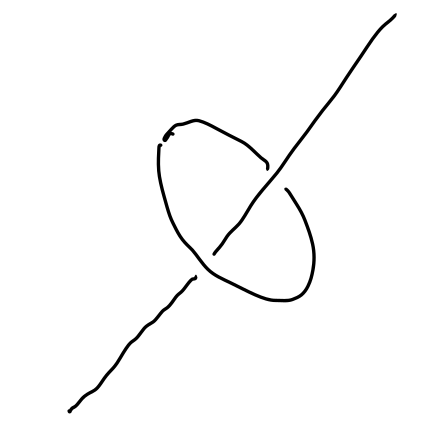
\includegraphics[width=2cm]{frilec1graphics/link.png}
\end{figure}

%\todo[inline]{Add figure!}

\subsection{General Structure of Line Operators}

Note that $Z(S^1)$ is a linear category, and objects $\ell \in Z(S^1)$ are used to ``firm up'' surfaces.
More precisely, if $\Sigma$ is a surface with holes, and to each hole we assign some $\ell_i \in Z(S^1)$, then we obtain a \emph{vector space} $Z(\Sigma; \ell_1, \dots, \ell_n)$.

Morphisms in $Z(S^1)$ are defined as follows.
Consider the cylinder $C = S^1 \times [0, 1]$ as having two incoming boundary components and no outgoing boundary.
If we place a line operator $\ell_i$ ($i = 1, 2$) at each boundary component,
we get %\todo{add figures!}
\begin{equation}
Z(C; \ell_1, \ell_2) = \Hom_{Z(S^1)}(\ell_1, \ell_2).
\end{equation}
This corresponds to the following cobordism:
\begin{figure}[htp]
    \centering
    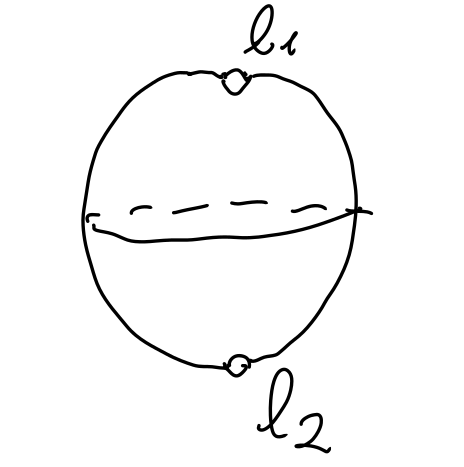
\includegraphics[width=3cm]{frilec1graphics/hom.png}
\end{figure}

\noindent We can view $Z(C)$ as the functor
\begin{equation}
Z(C) = \Hom_{Z(S^1)}(-, -).
\end{equation}

\noindent The product on $Z(S^2)$ comes from sticking small disks $D^3_1$, $D^3_2$ inside a larger disk $D^3$:
\begin{figure}[htp]
    \centering
    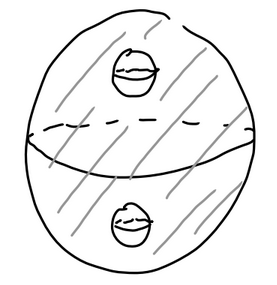
\includegraphics[width=3cm]{frilec1graphics/E3mult.png}
\end{figure}

\noindent This defines a cobordism $D^3 \setminus (\mathring{D}^3_1 \sqcup \mathring{D}^3_1): S^2_1 \sqcup S^2_2 \to S^2$
%\todo{add figure!}
which gives an $\E_3$ multiplication on $S^2$.

We can adapt this picture to get a description of composition of morphisms in $Z(S^1)$.
Namely, the surface (topologically a torus)
\begin{figure}[!htp]
    \centering
    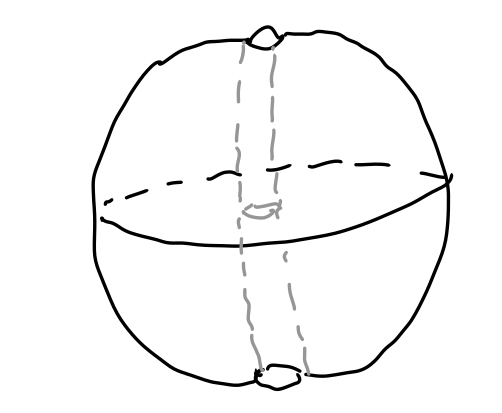
\includegraphics[width=3cm]{frilec1graphics/compos.png}
\end{figure}

\noindent defines the composition map
\begin{equation}
\circ: \Hom_{Z(S^1)}(\ell_2, \ell_3) \otimes \Hom_{Z(S^1)}(\ell_1, \ell_2) \to \Hom_{Z(S^1)}(\ell_1, \ell_3).
\end{equation}

The category $Z(S^1)$ has an $\E_2$-structure.
In other words, we can view $Z(S^1)$ as a braided tensor category.
This structure comes from the following morphisms:%\todo{add figures!}
\begin{itemize}
    \item A tensor operation $\otimes: Z(S^1) \boxtimes Z(S^1) \to Z(S^1)$ defined by
    \begin{figure}[htp]
    \centering
    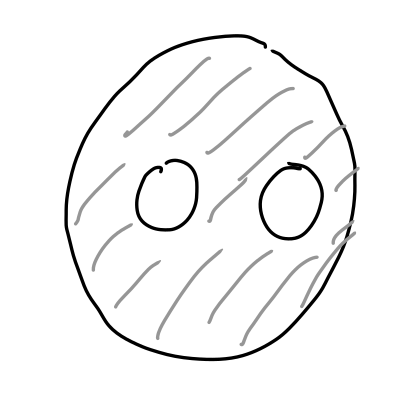
\includegraphics[width=3cm]{frilec1graphics/mult.png}
\end{figure}
    \item A braiding defined by
    \begin{figure}[htp]
    \centering
    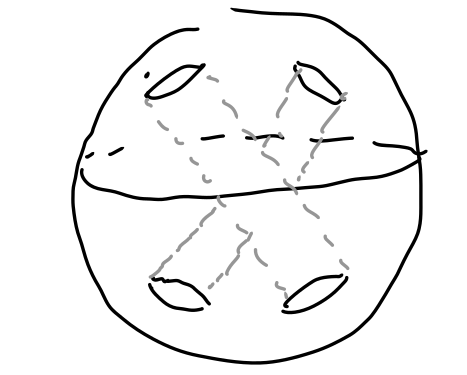
\includegraphics[width=3cm]{frilec1graphics/braiding.png}
\end{figure}
    \item A tensor unit $\mathbbm{1} \in Z(S^1)$, the \defterm{trivial} or \defterm{identity line}, defined by
    \begin{figure}[htp]
    \centering
    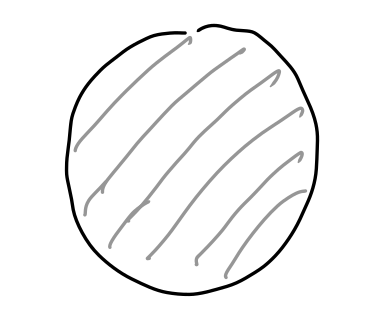
\includegraphics[width=3cm]{frilec1graphics/unit.png}
\end{figure}
\end{itemize}

The category $Z(S^1)$ has an $S^1$-action coming from the group $S^1$ acting on the manifold $S^1$ by rotation.
Passing to $S^1$-invariants (in physics language, ``turning on an Omega background'') takes us from an $\E_2$-category to an $\E_0$-category (i.e. a category with a distinguished object $\mathbbm{1}$).
One can compare this to how taking $S^1$-invariants sends the $\E_3$-algebra $Z(S^2)$ to an $\E_1$-algebra.

\subsection{State Spaces from $Z(S^1)$}

We can recover the value of $Z$ on a surface (or a $3$-manifold) from $Z(S^1)$.

\begin{example}
To compute $Z(S^2)$, we note
\begin{equation}
Z(S^2) = Z(D^2 \cup_{S^1} D^2) = \Hom_{Z(S^1)}(Z(D^2), Z(D^2)) = \Hom_{Z(S^1)}(\mathbbm{1}, \mathbbm{1}) = \mathrm{End}_{Z(S^1)}(\mathbbm{1}).
\end{equation}
From the physics of $3$d $\cN = 4$ gauge theories, we know that $Z(S^2) = \C[\cM_{\mathrm{vac}}]$.
If we know $\cM_{\mathrm{vac}}$ (or its affinization $\cM_{\mathrm{vac}}^{\mathrm{aff}}$), this gives us a good check for proposed definitions of $Z_A(S^1)$ and $Z_B(S^1)$.
\end{example}

Consider the functor\footnote{Here we are making explicit the previously implicit assumption that the categories appearing in the study of $3$d $\cN = 4$ gauge theories are all derived / dg-categories.}
\begin{equation}
\Hom_{Z(S^1)}(-, \mathbbm{1}): Z(S^1)^{\mathrm{op}} \to \C[\cM_{vac}]-\mod = \bfD^b\big(\mathrm{Coh}(\cM_{\mathrm{vac}}^{\mathrm{aff}})\big).
\end{equation}
If $\cM_{\mathrm{vac}}$ is smooth, renormalization group flow arguments tell us that this functor should be an equivalence.
In general, $Z(S^1)$ will contain more information than $\bfD^b\big(\mathrm{Coh}(\cM_{\mathrm{vac}}^{\mathrm{aff}})\big)$, e.g.\ $Z(S^1)$ controls deformations and resolutions of $\cM_{\mathrm{vac}}^{\mathrm{aff}}$.

\begin{example}
To compute $Z(T^2)$, we note
\begin{equation}
Z(T^2) = Z\big((S^1 \times [0, 1]) / ((x, 0) \sim (x, 1)\big) = \textrm{``trace of Hom''} := \mathrm{HH}_\bullet(Z(S^1)), 
\end{equation}
the Hochschild homology of the category $Z(S^1)$.
The ``trace'' here can be understood using the picture of beads on a string
\begin{figure}[htp]
    \centering
    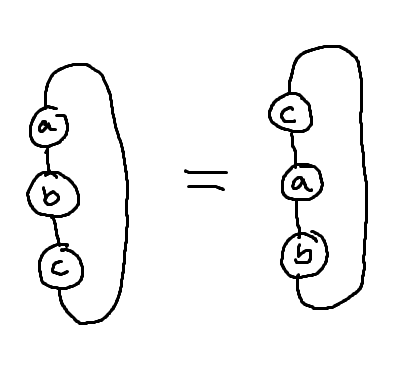
\includegraphics[width=3cm]{frilec1graphics/trace.png}
\end{figure}

\noindent where the ``beads'' (here $a, b, c$) are homomorphisms, and the picture defines the trace of the composite (here $\mathrm{tr}(abc) = \mathrm{tr}(cab)$).
\end{example}

\subsection{Line Operators in Topological Twists: Strategy}

To compute $Z(S^1)$ for the A- or B-twists of the $3$d $\cN = 4$ gauge theory corresponding to $G$ and $T^* V$ (where $\rho: G \to \mathrm{U}(V)$ is a unitary representation), we proceed by:
\begin{enumerate}
    \item Solving the equations of motion for the A- or B-twist.
    \item ``Quantizing,'' roughly by:
    \begin{enumerate}
        \item (A-twist) taking the Fukaya category of the moduli space of solutions.
        \item (B-twist) taking $\bfD^b \mathrm{Coh}$ of the moduli space of solutions.
    \end{enumerate}
\end{enumerate}
We will work this out in more detail as follows.

\subsection{Line Operators in the $3$d B-Model}

Fix coordinates $\vec{X}, \vec{Y}$ on $T^* V = V \oplus V^*$, and write a general $G_\C$-connection as $\cA$.
The equations of motion of the $B$-twist are given by setting $Q_B(-) = 0$ for all fields.
This yields:
\begin{equation}
    \begin{cases}
        \cF_\cA = 0 \\
        \mathrm{d}_\cA \vec{X} = \mathrm{d}_\cA \vec{Y} = 0 \\
        \mu_\C(\vec{X}, \vec{Y}) = \rho^*(\vec{X}, \vec{Y}) = 0 \\
        \textrm{a reality equation}
    \end{cases}
\end{equation}
To find the moduli space of solutions, we must quotient by $G$-gauge transformations.
In fact, it is more convenient to quotient by $G_\C$-gauge transformations, which removes the reality equation.

In an infinitesimal neighborhood of $S^1$ in $\R^3$, the only information in the connection $\cA$ is the holonomy $g = \mathrm{Hol}_{S^1_p}(\cA) \in G_\C$ for some point $p \in S^1$.
Let $\vec{X}_p$ and $\vec{Y}_p$ be the values of the fields $\vec{X}$ and $\vec{Y}$ at $p$.
Our equations of motion become
\begin{equation}
\begin{cases}
    g \vec{X}_p = \vec{X}_p \\
    \vec{Y}_p g^{-1} = \vec{Y}_p \\
    \mu_\C(\vec{X}_p, \vec{Y}_p) = 0.
\end{cases}
\end{equation}

It is a good exercise to check that these equations are equivalent to the single equation $\mathrm{d} W = 0$ for $W: G_\C \times V \times V^* \to \C$ given by
\begin{equation}
W(g, \vec{X}, \vec{Y}) = \vec{Y} \cdot (\rho(g) - 1) \vec{X}.
\end{equation}
Thus the moduli space of solutions is
\begin{equation}
\Big\{ \big(g, \vec{X}, \vec{Y}\big) \in G_\C \times V \times V^* \, \Big| \, \mathrm{d}_{(g, \vec{X}, \vec{Y})} W = 0 \Big\} / G_\C.
\end{equation}
Here $h \in G_\C$ acts by $h \cdot (g, \vec{X}, \vec{Y}) \mapsto (h g h^{-1}, h \vec{X}, \vec{Y} h^{-1})$.

The resulting moduli space is typically singular, so it is better to use the category of (equivatiant) matrix factorizations than the category of coherent sheaves.
Thus
\begin{equation}
Z^B_{G,V}(S^1) = \mathrm{MF}^{G_\C}\Big(\Big\{ \big(g, \vec{X}, \vec{Y}\big) \in G_\C \times V \times V^* \, \Big| \, \mathrm{d}_{(g, \vec{X}, \vec{Y})} W = 0 \Big\}\Big)
\end{equation}
Here $\mathbbm{1} = \cO_{g=1}$, and $\mathrm{End}(\mathbbm{1}) = \C[T^* V // G_\C] = \C[\cM_H]$.

\begin{example}
Consider the case where $G = 1$ and $V = \C$.
The moduli space of solutions is smooth in this case, so we can use coherent sheaves in place of matrix factorizations, and
\begin{equation}
Z^B_{1,\C}(S^1) = \bfD^b \mathrm{Coh}(T^* \C),
\end{equation}
Here $\mathbbm{1} = \O_{T^* \C}$ and $\mathrm{End}(\mathbbm{1}) = \C[T^* \C]$.

It is more interesting to note that
\begin{equation}
Z^B_{1,\C}(T^2) = \mathrm{HH}_\bullet(\bfD^b \mathrm{Coh}(T^* \C)) = \C[X, Y, \mathrm{d}\overline{X}, \mathrm{d}\overline{Y}]
\end{equation}
by the Hochschild-Kostant-Rosenberg theorem.
Here $X$ and $Y$ are in even degree, and $\mathrm{d}\overline{X}$ and $\mathrm{d}\overline{Y}$ are in odd degree.
\end{example}

\subsection{Line Operators in the $3$d A-Model}

If we think algebraically and ``squint hard enough,'' an infinitesimal neighborhood of $S^1$ in $\R^3$ looks like $D^\times = \mathrm{Spec} \C((z))$.
The moduli space solutions to the $3$d A-model equations of motion on $D^\times$ look like $T^*\big(V((z)) / G_\C((z)) \big)$, where the quotient by $G_\C((z))$ corresponds to modding out by gauge equivalence.

We expect $Z^A_{G,V}(S^1)$ to be something like the Fukaya category of this moduli space, but this is hard to define rigorously.
Work of Justin Hilburn and Philsang Yoo proposes that we instead consider the category of $D$-modules (or constructible sheaves) on the base of the cotangent bundle.
The modified proposal is then
\begin{equation}
Z^A_{G,V}(S^1) = D-\mod\big(V((z)) / G_\C((z))\big) = D-\mod^{G_\C((z))}\big(V((z))\big),
\end{equation}
the category of strongly equivariant $D$-modules on $V((z))$.

This definition may look abstract, but it is compatible with the BFN construction of Coulomb branches, providing evidence for its validity.
Basic objects of $Z^A_{G,V}(S^1)$ are labeled by pairs
\begin{equation}
\{ (L \subset V((z)) \textrm{ a subspace}, H \subset G_\C((z))\textrm{ a subgroup}) \, | \, H \textrm{ stabilizes } L \}.
\end{equation}
Here
\begin{align}
\Hom_{Z^A_{G,V}(S^1)}\big((L, H), (L', H')\big) &= \mathrm{H}_\bullet((L' / H') \times_{V((z)) / G_\C((z))} L / H) \\
&= \mathrm{H}_\bullet \left(H' \backslash \{ (\vec{X}, \vec{X}', g) \in L \times L' \times G_\C((z)) \, | \, \vec{X}' = g \vec{X} \} / H\right).
\end{align}
The unit object $\mathbbm{1}$ is given by the pair $(V[[z]], G_\C[[z]])$ (this is an algebraic version of ``filling in $D^\times$ to $D$'').
One can check that $\mathrm{End}(\mathbbm{1}) = \C[\cM_C]$, as claimed above.

\subsection{$3$d Mirror Symmetry for Line Operators}

Mirror symmetry results have been proven for categories of line operators in the case when $G$ is abelian.
We discuss some of them here.

\begin{Theorem}[Hilburn, Raskin]
There exists an equivalence of categories between $Z^A_{1,\C}(S^1)$ and a de Rham version of $Z^B_{U(1), \C}(S^1)$.
\end{Theorem}

This theorem can be extended to other examples by looking at the behavior of the tensoring operation and the action of hyperk\"ahler isometries.

Another approach proceeds by interpreting line operators in terms of vertex algebras.

\begin{Theorem}[Ballin, Creutzig, Dimofte, Niu]
If $G$ is abelian and $G \curvearrowright V$ is faithful, then
\[
Z^B_{G,V}(S^1)^{\mathrm{finitely \,\, supported \,\, on \,\,} G_\C} \simeq \bfD^b(\mathrm{modules \,\, over \,\, some \,\, VOA})
\]
as braided tensor categories.
Furthermore, there is a $3$d mirror symmetry statement relating this to an A-side category of VOA modules contained in $Z^A_{G^!,V^!}(S^1)$.
\end{Theorem}

The slogan of this theorem is that $3$d mirror symmetry for line operators looks like $2$d mirror symmetry on loop spaces.

The nonabelian case is poorly understood, and work on understanding it is highly desirable.
One viewpoint on the nonabelian case comes from Ben Webster's work interpreting $3$d mirror symmetry combinatorially using KLRW algebras.

\begin{Theorem}[Webster]
When $\cM_C$ admits a full resolution $\widetilde{\cM_C} \to \cM_C$, there exists a deformation of $Z^A_{G,V}(S^1)$ to $\bfD^b\big(\mathrm{Coh}(\widetilde{\cM_C})\big)$.
\end{Theorem}

This is a non-abelian mirror symmetry statement, but it misses information about the singularities.
The deformation here is mirror to the deformation of $Z^B_{G^!, V^!}(S^1)$ obtained by imposing GIT stability parameters.
It would be good to have an improved version of this theorem incorporating the full category of line operators in the $A$-model and singularities of the moduli space.

\subsection{Exercises}

\begin{exercise}
Suppose that $G=U(1)$ acts on $V=\C^2$ with weights $(1,3)$. (In other words $e^{i\theta}:(X^1,X^2)\mapsto (e^{i\theta}X^1,e^{3i\theta}X^2)$.)

Write down explicitly the superpotential
%
$$  W : G_\C \times V \times V^* \to \C $$
%
that appears in the solution to the B-twist equations of motion on $S^1$. Differentiate with respect to $g\in G_\C$ to recover the complex moment map $\mu_\C$ for the action on $T^*V$.

\end{exercise}

For the remaining problems, recall that in the A twist of $(G,T^*V)$ gauge theory, the category $Z(S^1)$ has (some) objects labelled by $(L,H)$ where $L$ is a subspace of $V(\!(z)\!)$, and $H$ is a subgroup of $G_\C(\!(z)\!)$ that stabilizes $L$. The morphism space between two such objects may be defined as Borel-Moore homology
%
$$ \text{Hom}\big((L,H),(L',H')\big) := H_\bullet\Big(  H'\big\backslash\big\{ (X',X,g)\in L'\times L\times G_\C(\!(z)\!)\,\big|\, X'=gX\big\}\big/H \Big) $$
%
Note that when a quotient is not free (as in the $H$ or $H'$ quotients above) it should be interpreted as taking equivariant cohomology.

\begin{exercise}

Let $1\!\!1 := (V[\![z]\!],G_\C[\![z]\!])$. Argue that $\text{End}(1\!\!1) = \C[\cM_C]$ reproduces the BFN construction of the Coulomb branch.

\end{exercise}

\begin{exercise}
Take $G=U(1)$ and $V=\C$ (with weight $1$). Recall that the Coulomb branch algebra may be presented as
%
$$ \C[\cM_\C] \simeq \C[v_+,v_-,\varphi]/(v_+v_-=\varphi)\,. $$
\end{exercise}
%
Consider line operators
%
$$ \cN_+ = (\C(\!(z)\!),\C(\!(z)\!)^*)\,,\qquad  \cN_- = (0,\C(\!(z)\!)^*)\,. $$
%
Show that they give rise to modules
%
$$ \text{Hom}(\cN_+,1\!\!1) = \C[\cM_C]/(v_+-1)\,,\qquad \text{Hom}(\cN_i,1\!\!1) = \C[\cM_C]/(v_--1)\,. $$

\end{document}

\section{Lecture 16 (Friday)}
% \input{frilec2}

\section{Lecture 17 (Friday)}
% \input{frilec3}

\section{Lecture 18 (Friday)}
% 
\subsection{Quiver gauge theories}

Dualizing exact sequences appears many times in \textit{abelian} 3D mirror symmetry. \textit{Nonabelian} 3D mirror symmetry however is not as systematic. Not all gauge theories have gauge theory mirrors. There are rich families of mirror pairs, but they all come from string/M theory. 

We form generalized quiver gauge theories from \textit{unitary quivers}, and get $3D, N=4$ theories. 

\begin{definition}
A unitary quiver is an unoriented graph with circle or square nodes 
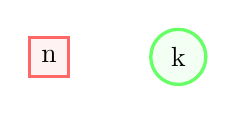
\begin{tikzpicture}[
roundnode/.style={circle, draw=green!60, fill=green!5, very thick, minimum size=7mm},
squarednode/.style={rectangle, draw=red!60, fill=red!5, very thick, minimum size=5mm},
]
%Nodes
\node[squarednode]  (maintopic)  {n};
\node[roundnode]  (rightsquare)  [right=of maintopic] {k};
\end{tikzpicture}
labelled by $k,n \in \mathbb{N}$, and edges between nodes. Attached to each circle node $v$ is the unitary group $U(n_v)$, where $n_v$ is the labelling of $v.$ Take the gauge group of the quiver to be the product over circle nodes $G = \prod_{\textit{circle nodes }v} U(n_v)$ and the representation space to be $W = \oplus_{v \rightarrow v'} (Hom(\bC^{n_v}, \bC^{n_{v'}}) \oplus Hom(\bC^{n_{v'}}, \bC^{n_v}))$.
\end{definition}

\begin{example}
Consider the following quiver $\Gamma.$
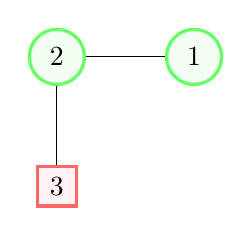
\begin{tikzpicture}[
roundnode/.style={circle, draw=green!60, fill=green!5, very thick, minimum size=7mm},
squarednode/.style={rectangle, draw=red!60, fill=red!5, very thick, minimum size=5mm},
]
%Nodes
\node[roundnode]      (maintopic)                              {2};
\node[roundnode]      (rightsquare)       [right=of maintopic] {1};
\node[squarednode]    (lowersquare)       [below=of maintopic] {3};

%Lines
\draw[-] (maintopic.east) -- (rightsquare.west);
\draw[-] (maintopic.south) -- (lowersquare.north);
\end{tikzpicture}
The gauge group is $U(2) \times U(1).$ Take $W = T^*(Hom(\bC, \bC^2) \oplus Hom(\bC^2, \bC^3))$. The Higgs branch $\mathcal{M}_H(\Gamma)$ of $\Gamma$ is the Nakajima quiver variety associated to $\Gamma.$ The Coulomb branch $\mathcal{M}_C(\Gamma)$ is the nilpotent cone $Nilp(\mathfrak{sl}_3)$, which is resolved by $T^* Flag(\mathfrak{sl}_3)$. In fact $\mathcal{M}_C \cong \mathcal{M}_H$, so this quiver is self-mirror.
\end{example}

We have two families of non-abelian dualities:

\textbf{Family 1:} 11-dimensional M theory with $n$ M2 branes $\mathbb{R}^3 \times 0 \times 0$ on Kleinian singularities $\mathbb{R}^3 \times \bC^2/K_1 \times \bC^2/K_2$, where $K_1, K_2$ are discrete subgroups of $SU(2)$. The Higgs branch is $\mathcal{M}_H = \{\textit{n }  ADE(K_1)$ instantons on $\bC^2/K_2\}$, and the Coulomb branch $\mathcal{M}_C$ is defined in the same way with $K_1$ and $K_2$ swapped. Concretely, suppose we have $\mathbb{R}^3 \times \bC^2/\mathbb{Z}_k \times \bC^2/\mathbb{Z}_l$. Take the quiver $\Gamma$ to be the necklace of $l$ circle nodes, each decorated by $n$, with a single square node decorated by $k$ connecting to a single circle node. The 3D-mirror quiver $\Gamma'$ is the necklace of $k$ circle nodes, each decorated by $n$ with a single square node decorated by $l$ connecting to a single circle node. The Higgs branch is $\{\textit{n } U(k) $ instantons on $\bC^2/\mathbb{Z}_l\}$ and the Coulomb branch is with $k$ and $l$ swapped.

Take $k=l=1$. Then $G = U(n), W = \mathfrak{gl}_n \oplus \mathbb{C}^n$ and $\mathcal{M}_H = Sym^n(T^*\mathbb{C}) \cong \mathcal{M}_C$. "Quantizing the Hilbert scheme $\rightarrow$ Cherednik algebras"

\textbf{Family 2:}  D3 branes (ending on D5) in IIB string theory, Gaiotto-Witten "S-duality, boundary conditions...". Hanany-Witten moves provide an extremely efficient way to produce mirror theories. Also there are Nakajima bow varieties...

\begin{example}
Take
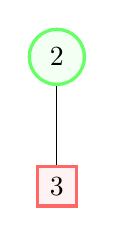
\begin{tikzpicture}[
roundnode/.style={circle, draw=green!60, fill=green!5, very thick, minimum size=7mm},
squarednode/.style={rectangle, draw=red!60, fill=red!5, very thick, minimum size=5mm},
]
%Nodes
\node[roundnode]      (maintopic)                              {2};
\node[squarednode]    (lowersquare)       [below=of maintopic] {3};

%Lines
\draw[-] (maintopic.south) -- (lowersquare.north);
\end{tikzpicture}
The gauge group is $G = U(2), W = \bC^2 \otimes \bC^4$. The Higgs branch $\mathcal{M}_H$ is $T^*Gr(2,4).$
\end{example}

A major open problem is defining (almost) all levels in $Z^A, Z^B$ TQFTs for non-abelian theories! The things we do know are very little,
\begin{enumerate}
\item $Z(S^2)$ (but what is the HK metric on $\mathcal{M}_C$?)
\item Symplectic duality folowing Webster, i.e. when $\mathcal{M}_C, \mathcal{M}_H$ have smooth symplectic resolutions
\item From $Z^A_{G, V}(S^1)$ to $D^bCoh(\mathcal{M}_C^{res})$
\end{enumerate}
We want to define $Z(\Sigma_g), Z(S^1), Z(pt)$ for non-abelian theories and prove mirror symmetry.

There are multiple constructions using derived algebraic geometry, analysis, vertex operator algebras (VOAs). In the last $Z_{A/B}(\Sigma_g) = $ conformal blocks of a VOA (Costello-Gaiotto). 

Even for abelian theories, we would love to see complete 3-2-1-0 TQFT with definitions matching at all levels.

There exists another twist! The holomorphic topological twist $Q_{HT}.$ This is related to elliptic cohomology, elliptic stable envelopes, vertex functions.

With $G, T^* V, \mathcal{M}_H^{res} = T^*V//G$ with $\mu_{\mathbb{R}} \neq 0$, the elliptic cohomology gives $Z_{G, V}^{HT}(T^2).$

Elliptic stable envelopes are $Z_{G,V}^{HT}(D^2 \times S^1) \cong Z_{G^{\vee}, V^{\vee}}^{HT}(D^2 \times S^1)$ with boundary condition $\alpha$ given by $D^2$, [Aganagic-Okounkov].

Also, there's know homology. Teleman: "Gauge theory and Mirror Symmetry", $G$-actions on the Fukaya category.

Quantum K-theory is defined for K\"ahler manfolds $(N=2)$, no need for hyperK\"ahler structure $(N=4).$ In 2D, A-twist, target K\"ahler, $Z(S^1) = QH^{\cdot}(X).$ In 3D, $N=2$ $\sigma$-model to $X$, we have $Q^{HT}$ and quantum K-theory is given by $Z_X^{HT}(S^1 \times S^1) = QK^{\cdot}(X).$

Also some final words about vertex operator algebras, Kac-Moody, magnetic quivers.

\end{document}

\end{document}
